\section{Classical and Quantum Low-degree Tests}
\label{sec:ldt}

In this section we introduce the classical and quantum low individual degree tests, that form the basis of our classical, quantum-sound and quantum PCP constructions. For quantum soundness of the classical test we refer to~\cite{ML20}. For the quantum test, we refer to~\cite{natarajan2018low} and its adaptation to the low individual degree test given in Appendix~\ref{sec:qld-analysis}. 
The protocol in this work combines both of these tests, using the quantum
low individual degree test for question reduction and the classical low individual degree test for
answer reduction.
Section~\ref{sec:ld-verifier} below introduces the classical test,
and Section~\ref{sec:pauli-verifier} does the same for the quantum 
test.
Prior to doing this, we introduce the \emph{Magic Square game} in
Section~\ref{sec:ms}, a key subroutine in the quantum test.


\subsection{The classical low-degree test}
\label{sec:ld-verifier}

We begin with a generalization of the classical low-degree test known as the
``simultaneous individual low-degree test''.
We sometimes refer to this as the ``classical low-degree test'' for short.
The low-degree test is used as a subroutine in the Pauli Basis test (see
Section~\ref{sec:pauli-verifier}) as well as the answer-reduction normal form
verifier (see Section~\ref{sec:ans}).
We describe the test as a nonlocal game in Section~\ref{sec:ld-game} and show
that the question distribution can be implemented as a (typed) conditionally
linear distribution (see \Cref{sec:types} for the definition of typed CL
distributions).


\subsubsection{The game}
\label{sec:ld-game}

The game $\game^\ld$ is parametrized by a tuple $\ldparams = (q, m, d, \ldc)$
where $m, d, \ldc \in \N$ are integers, $q \in \N$ is an admissible field size,
and $m$ divides $q$.
We sometimes write $\game^\ld_\ldparams$ to emphasize the dependence of the
classical low-degree test on the parameter tuple $\ldparams$.

We first provide a high-level description of the game for $k=1$.
It is based on the low-individual degree variant of the multilinearity test
of~\cite{babai1991non}, where one player (called the ``points player'') receives
a random point $u \in \F_q^m$, and the other player (called the ``lines
player'') receives a random axis-parallel line $\line$ that contains $u$, i.e.\
the line parallel to the $i$-th axis which goes through point $u$, for uniformly
random $i\in\{1,\ldots,m\}$.
The points player is supposed to respond with a value $a \in \F_q$, and the
lines player is supposed to respond with a univariate polynomial $f_\line$ of
degree at most $d$ such that $f_\line(u_i) = a$, where $u_i$ is the $i$-th
coordinate of $u$.

Suppose the players agree beforehand on a global polynomial $g: \F_q^m \to \F_q$
such that every variable has degree at most $d$.
Then a winning strategy is the following: the points player responds with
$g(u)$, and the lines player responds with the univariate polynomial $f_\line$
that is the restriction of $g$ to line $\line$; formally, for $t \in \F_q$,
\[f_\line(t)=g(u_1,u_2,\ldots,u_{i-1},t,u_{i+1},\ldots,u_m)\;.\] It is easy to
see that $f_\line(t)$ has degree at most $d$ in the variable $t$.
Thus in this case the players will pass the low-degree test with probability
$1$.
The low-degree testing theorem states that the converse approximately holds: if
the players pass the low-degree test with probability close to $1$, then their
responses must be approximately consistent (in some sense) with a global
polynomial $g$ with individual degree $d$.

When $k > 1$, the players are supposed to respond with a \emph{tuple} of
answers; and the test is intended to check that the players' responses are
consistent with a $k$-tuple of functions $g_i: \F_q^m \to \F_q$ that are
polynomials where every variable has degree at most $d$.

The game that we use is slightly more elaborate than the ``axis-parallel
lines-versus-points'' test just described.
In addition, we have two other subtests.
One is a ``diagonal line-vs-points'' test: here, the points player receives a
point $u \in \F_q^m$ as before, but the lines player receives a line $\line$
that goes through $u$ but is not necessarily axis-aligned.
Instead, it's chosen by first picking an index $i \in \{1,2,\ldots,m\}$
uniformly at random, picking $v \in \F_q^m$ uniformly at random, and letting $v'
= \pi_{i-1}(v) = (0,0,\ldots,0,v_i,v_{i+1},\ldots,v_m)$ (i.e., $\pi_{i-1}$
zeroes out the first $i-1$ coordinates of its input).
Then, the line is defined as the set
\[
	\line = \{ u + tv' : t \in \F_q \}\;,
\]
which is a uniformly random line in the affine subspace of $\F^m_q$
corresponding to all points $v$ whose first $(i-1)$ coordinates match those of
$u$.
The points player responds with a value $a \in \F_q$, the lines player responds
with a univariate polynomial $f_\line$ of degree $md$,\footnote{Since $\line$ is
  no longer axis-parallel, the restriction of an individual degree-$d$
  polynomial $g$ to a line $\line$ may yield a degree $md$ polynomial.}
and the verifier checks that $f_\line(t_u) = a$ (where $t_u \in \F_q$ is the
projection of $u$ onto the line $\line$ with respect to a canonical
parameterization of $\line$).

The other additional test is a ``consistency test'', where both players receive
either the same points question, the same axis-parallel lines question, or the
same diagonal lines question.
In all cases they are expected to respond with the same answer.



\paragraph{Axis-parallel lines and diagonal lines.}
Before presenting a formal description of the game $\game^\ld$, we first define
what we mean by lines, and their properties.

\begin{definition}[Lines]
  \label{def:line}
	A \emph{line} $\line$ in $\F^m_q$ specified by a pair $(u,v) \in (\F_q^m)^2$
  is the subset
  \begin{equation}
    \label{eq:line-set}
    \line(u,v) = \bigl\{\, u + tv : t \in \F_q \,\bigr\} \subseteq \F_q^m \;.
  \end{equation}
  We call the vector $v$ a \emph{direction} of line
  $\line(u,v)$.\footnote{For convenience we explicitly allow
    $v=0$, in which case the line is reduced to a singleton.}
  
  A line $\line(u,v)$ is \emph{axis-parallel} if there is a coordinate $i \in
  \{1,2,\ldots,m\}$ for which $v$ is equal to $e_i$, the $i$-th elementary basis
  vector in $\F_q^m$.
  We say that such a line $\line$ is \emph{parallel to the $i$-th direction}.
  A line $\line(u,v)$ is \emph{diagonal} if there exists an $i \in
  \{0,1,\ldots,m-1\}$ for which $v_1 = v_2 = \cdots = v_i = 0$.
\end{definition}

The following Proposition establishes that, for a fixed direction, a line
$\line$ is an equivalence class of points on the line.
\begin{proposition}
  \label{prop:line-equiv}
  Let $u,v \in \F_q^m$.
  Then for all $u' \in \line(u,v)$, we have that $\line(u,v) = \line(u',v)$.
\end{proposition}
\begin{proof}
	Fix $u' \in \line(u,v)$.
  We have that $u' = u + tv$ for some $t \in \F_q$.
  Let $a \in \line(u,v)$.
  This means that $a = u + sv$ for some $s\in \F_q$.
  We also have that $a = u + (s - t + t)v = u + tv + (s - t)v = u' + (s - t)v$,
  so $\line(u,v) \subseteq \line(u',v)$.
  A similar argument shows that $\line(u',v) \subseteq \line(u,v)$.
\end{proof}

We now specify a canonical representation of lines $\line = \line(u,v)$ as pairs $(u_0,v)$
where $u_0$ is a \emph{canonical representative} of $\line$ specified as
follows.
Let $L_v^{\lnf}: \F_q^m \to \F_q^m$ denote the canonical linear map with the
one-dimensional kernel basis $\{v\}$ (see \Cref{def:cl-canonical} for a
definition of canonical linear map).
Note that for all $u \in \line$, we have that $L_v^{\lnf}(u)$ is a point in
$\line$.
This is because since the image and kernel of $L_v^{\lnf}$ are complementary
subspaces by definition (see \Cref{def:cl-canonical}), any $u \in \F_q^m$ has a
unique decomposition $u = u_0 + u_1$ where $u_0$ is in the image of $L_v^{\lnf}$
and $u_1 \in \ker(L_v^{\lnf})$, which by definition is the subspace spanned by
$v$.
Thus $u_1 = tv$ for some $t \in \F_q$ and we have that $u_0 = u - tv \in \line$.
In particular, if $u\in \line$ then $u_0 = L_v^{\lnf}(u) \in \line$ as well. 
Furthermore, since $L_v^{\lnf}$ is a projection onto its image by definition, we
have $L_v^{\lnf}(u_0) = u_0$.

Next, note that for any $u,u' \in \line$, since $u-u' = sv$ for some $s\in \F_q$
it follows that $L_v^\lnf(u) = L_v^\lnf(u')$.
Thus $u_0 = u_0'$ and this shows that $L_v^\lnf$ gives a means to compute a
canonical representative of lines.

\begin{definition}[Canonical representative of a line]
  \label{def:line-representative}
  Let $\line$ be a line in direction $v$.
  A canonical representative of $\line$ is the point $u_0 \in \F_q^m$ such that
  \[
    u_0 = L_v^\lnf(u)
  \]
  for all $u \in \line$.
\end{definition}



\paragraph{Question distribution.}
We now present the question distribution of the game $\game^\ld$ as a typed CL
distribution (see \Cref{sec:types} for the definition of typed CL functions and
typed CL distributions).
The type set $\type^\ld$ of the game $\game^\ld$ we use is
\[
	\type^\ld = \{ \Point, \ALine, \DLine \}\;.
\]
The distribution over question types is uniform over $\type^\ld \times \type^\ld$. 

We introduce the corresponding typed CL functions $L_\Point$, $L_\ALine$,
$L_\DLine$ where the corresponding CL distributions $\mu_{L_\ALine,L_\Point}$
and $\mu_{L_\DLine,L_\Point}$ implement the axis line-versus-point and diagonal
line-versus-point distributions, respectively.
The functions are parametrized by a field size $q$, a dimension $m$, and three
complementary register subspaces $V_\xpt,V_{\coord}, V_{\dir{}}$ of some ambient
space.
The register $V_\xpt$ (which is isomorphic to $\F_q^m$) is called the
\emph{point register}, $V_\coord$ (which is isomorphic to $\F_q$) is called the
\emph{coordinate register}, and $V_{\dir{}}$ (which is isomorphic to $\F_q^m$)
is called the \emph{direction register}, respectively.
We let $V$ denote the direct sum $V_\xpt \oplus V_{\coord} \oplus V_{\dir{}}$.
We identify elements of $V$ as triples $(u,s,v) \in \F_q^m \times \F_q \times
\F_q^m$.

Define $L_\Point$ to be the $1$-level CL function that projects onto $V_\xpt$: for every $(u,s,v) \in V$,
\begin{equation}
  \label{eq:cl-ptf}
	L_\Point(u,s,v) = (u,0,0) \;.
\end{equation}
Define $L_\ALine$ to be the following $2$-level CL function:
\begin{equation}
  \label{eq:cl-alnf}
	L_\ALine(u,s,v) = (L^\lnf_{e_i}(u), s, 0)\ \text{for all } (u,s,v) \in V,
\end{equation}
where $L^\lnf$ is the linear function used to compute the canonical
representative of lines (see \Cref{def:line-representative}), and $i = \chi(s)$
where we define $\chi(s)$ to be the unique integer such that
\begin{equation}
\label{eq:chi-func}
	s = (\chi(s) - 1) \frac{q}{m} + r
\end{equation}
for some $0 \leq r < q/m$, and we interpret the field element $s \in \F_q$ as an
integer between $0$ and $q - 1$).
The function $L_\ALine$ is the concatenation of the $1$-level CL function that
projects the subspaces $V_{\coord} \oplus V_{\dir{}}$ down to $V_\coord$ (i.e.
zeroes out the entire $V_{\dir{}}$ register), and the family of $1$-level CL
functions $\{L^\lnf_{e_i} \}$ acting on $V_\xpt$, indexed by $i \in
\{1,2,\ldots,m\}$.
(See \Cref{lem:cl-concat} for definition of CL function concatenation.)
Thus $L_\ALine$ is a $2$-level CL function.

Define $L_\DLine$ to be the following $3$-level CL function: for all $(u,s,v) \in
V$,
\begin{equation}
\label{eq:cl-dlnf}
	L_\DLine(u,s,v) = (L^\lnf_{\pi_{i-1}(v)}(u),s,\pi_{i-1}(v))
\end{equation}
where $i = \chi(s)$.
The function $L_\DLine$ is the concatenation of the following CL functions (again, see \Cref{lem:cl-concat} for definition of CL function concatenation): (i) the identity function on $V_{\coord}$ (which is a $1$-level CL function); (ii) for every $i \in \{1,2,\ldots,m\}$ the $1$-level CL function on $V_{\dir{}}$ that maps $v \mapsto \pi_{i-1}(v)$ (i.e.~it zeroes out the first $i-1$ coordinates of $v$), and (iii) for every pair $(s,v') \in V_\coord \oplus V_{\dir{}}$, the $1$-level CL function $L^\lnf_{v'}$ acting on $V_\xpt$. Thus $L_\DLine$ is a $3$-level CL function.


The following two lemmas establish that the CL functions
$L_\Point,L_\ALine,L_\DLine$ give rise to the axis-parallel line-versus-point and
diagonal line-versus-point distributions.
\begin{lemma}
	\label{lem:alnf}
	Consider the pair $(\line, u)$ sampled in the following way: first, sample the
  tuple $((u_0,s,0),(u,0,0))$ from the CL distribution $\mu_{L_\ALine,L_\Point}$,
  and let $\line = \line(u_0,e_i)$ where $i = \chi(s)$.
  Then $u$ is a uniformly random point in $\F_q^m$ and $\line$ is a line that
  goes through $u$ and is parallel to a uniformly random axis $i \in
  \{1,2,\ldots,m\}$.
\end{lemma}
\begin{proof}
	Since $s$ is uniformly random in $\F_q$ and $m$ divides $q$ by assumption, we
  have that $i$ is uniformly random between $\{1,2,\ldots,m\}$ and therefore
  $(u_0,s)$ specifies a uniformly random axis-parallel line $\line(u_0,e_i)$.
  Since $u_0 = L^{\lnf}_{e_i}(u)$, we have that $u \in \line(u_0,e_i)$.
\end{proof}



\begin{lemma}
	\label{lem:dlnf}
	Consider the pair $(\line,u)$ sampled in the following way: first, sample the
  tuple $((u_0,s,v),(u,0,0))$ from the CL distribution $\mu_{L_\DLine,L_\Point}$,
  and let $\line = \line(u_0,v)$ where $i = \chi(s)$.
  Then $u$ is a uniformly random point in $\F_q^m$ and $\line$ is a random
  diagonal line that goes through $u$ and shares the first $i-1$ coordinates
  with $u$, for uniformly random $i$.
\end{lemma}
\begin{proof}
	The proof of this follows identically to \Cref{lem:alnf}.
\end{proof}

For later convenience we make the following definition. 

\begin{definition}[Line-point distributions]
        \label{def:line-point-dist}
 The \emph{axis line-point distribution} $D_{\ALine}$ is the
 distribution $\mu_{L_\ALine,L_\Point}$ over pairs $(\ell=(u_0,e_i),u)$
 (we omit the $0$ elements for simplicity). The \emph{diagonal
   line-point distribution} $D_{\DLine}$ is the distribution
 $\mu_{L_\DLine,L_\Point}$  over $(\ell=(u_0,s,v),u)$. The
 \emph{line-point distribution} $D_{\Line}$ is the equal mixture of the axis-parallel line-point distribution and the diagonal line-point distribution.
 In other words, a sample from $D_{\Line}$ is distributed as follows:
 with probability $\tfrac{1}{2}$, output a sample from $D_{\ALine}$,
 and with probability $\tfrac{1}{2}$, output a sample from $D_{\DLine}$.
\end{definition}
































\paragraph{Decision procedure} The decision procedure $\decider^\ld$ for the
game $\game^\ld$ is presented in Figure~\ref{fig:ld-decider}.
The table at the top specifies a parsing scheme for the questions and answers,
depending on the type of question.
For example, when a player receives a question with type $\Point$, the question
content $x$, a bit string of length $m \log q$, should be interpreted by the
decision procedure and the players as an element of the vector space $\F_q^m$,
as indicated in Section~\ref{sec:ff-representations}.
Similarly the answer to a question with type $\Point$ is expected to be a bit
string of length $\ldc \log q$, and is interpreted as an element of $\F_q^\ldc$.
For questions with type $\ALine$, the question content is a $(m \log q + \log
q)$-bit string, which is parsed as a pair $(u_0, s) \in \F_q^m \times \F_q$,
which in turn can be interpreted as a specification for an axis-parallel line
$\line(u_0,e_i)$ in $\F_q^m$ where $i = \chi(s)$, as described in
\Cref{lem:alnf}.
The answer is interpreted as the description of $\ldc$ degree-$d$ univariate
polynomials defined on the line $\line(u_0,e_i)$, each polynomial given by a
list of $d+1$ coefficients.
For questions with type $\DLine$, the question content is a $(2m \log q + \log
q)$-bit string, which is parsed as a triple $(u_0, s, v) \in \F_q^m \times \F_q
\times \F_q^m$ that specifies a diagonal line $\line(u_0,v')$ where $v' =
\pi_{i-1}(v)$ as described in \Cref{lem:dlnf}.
The answer is interpreted as the description of $\ldc$ degree-$md$ univariate
polynomials defined on the line $\line(u_0,v')$.
If the answers returned by the players do not fit this format the decision
procedure rejects.


\begin{figure}[!htbp]
  \centering
  \begin{gamespec}
    \setlength{\tabcolsep}{1em}
    \begin{tabularx}{\textwidth}{ l   l   X   }
      \toprule
      Type & Question Content & Answer Format \\
      \midrule
      $\Point$ & $ u \in \F_q^m$ & Element of $\F_q^\ldc$  \\
      $\ALine$ & $ (u_0, s) \in \F_q^m \times \F_q$ &
      $\ldc$ degree-$d$ polynomials $f_j: \F_q \to \F_q$\\
      $\DLine$ & $(u_0, s, v) \in \F_q^m \times \F_q \times \F_q^m$ & 
      $\ldc$ degree-$md$ polynomials $f_j: \F_q \to \F_q$\\
      \bottomrule
    \end{tabularx}

    \vspace{1em}

    Input to $\decider^\ld$: $(\tvar_\alice,x_\alice, \tvar_\bob, x_\bob,
    a_\alice, a_\bob)$.
    In all cases where no action is indicated, accept.
    For $w \in \AB$,

    \begin{enumerate}
      \setlength\itemsep{1pt}
    \item (\textbf{Consistency test}) If $\tvar_\alice = \tvar_\bob$, accept iff
      $a_\alice = a_\bob$.
    \item (\textbf{Axis-parallel line-versus-point test}) If $\tvar_w = \ALine$
      and $\tvar_{\overline{w}} = \Point$, accept iff $f_j(t) =
      (a_{\overline{w}})_j$ for all $j \in \{1,2,\ldots,\ldc\}$ where $t \in
      \F_q$ is such that $x_{\overline{w}} = u_0 + te_i$ where $i = \chi(s)$.
      
    \item (\textbf{Diagonal line-versus-point test}) If $\tvar_w = \DLine$ and
      $\tvar_{\overline{w}} = \Point$, accept iff $f_j(t) =
      (a_{\overline{w}})_j$ for all $j \in \{1,2,\ldots,\ldc\}$ where $t \in
      \F_q$ is such that $x_{\overline{w}} = u_0 + tv'$, where $v' =
      \pi_{i-1}(v)$ with $i = \chi(s)$.
    \end{enumerate}
  \end{gamespec}
  \caption{The decision procedure $\decider^\ld$ for the simultaneous low-degree
    test, parameterized by $\ldparams = (q,m,d,\ldc)$.
    The function $\chi(s)$ is defined in \Cref{eq:chi-func}, and $\pi_{i-1}(v)$
    zeroes out the first $i-1$ coordinates of $v$.}
  \label{fig:ld-decider}
\end{figure}

We define a special class of measurements that are relevant to the soundness
properties of the low-degree test.

\begin{definition}[Low-degree polynomial measurements]
  \label{def:ld-meas}
  Define $\polymeas{m}{d}{q}$ to be the set of POVM measurements whose outcomes
  correspond to (individual) degree-$d$ polynomials of $m$ variables over
  $\F_q$.
  More generally, for an integer $\ldc$ and tuples $m=(m_1, m_2, \ldots,
  m_\ldc)$, $d=(d_1, d_2, \ldots, d_\ldc)$ and $q=(q_1, q_2, \ldots, q_\ldc)$,
  we let $\simulpolymeas{m}{d}{q}{\ldc}$ be the set of measurements $G =
  \{G_{g_1,\, g_2,\, \ldots\,,\, g_\ldc}\}$ such that for $i\in\{1, 2, \ldots,
  \ldc\}$, $g_i$ is a polynomial $g_i:\F_{q_i}^{m_i} \rightarrow
  \F_{q_i}$ with individual degree $d_i$ (see \Cref{sec:ld-encoding} for a definition of individual degree). 
\end{definition}

Quantum soundness of a version of the classical low-degree test for polynomials of low \emph{total} degree was claimed
in~\cite{natarajan2018low}, building on an analysis of a three-prover version of the test in~\cite{vidick2016three}. Unfortunately there is a gap in the soundness analysis of this test. For our construction we use the low individual degree test, whose quantum soundness is shown in~\cite{ML20} and generalized in~\cite{ji2021quantum}. We state the result in the form that is most directly useful for us, and show how the stated result follows from~\cite{ji2021quantum}.

\begin{theorem}[Quantum soundness of the simultaneous classical low-degree test]
  \label{lem:ld-soundness}
  There exists a function $\delta_{\ld}(\eps, q, m, d, \ldc) = a (dm \ldc)^a (\eps^b + q^{-b} + 2^{-bmd})$ for universal constants $a\geq 1$ and $0<b\leq 1$ 
such that the following
  holds.
  For all $\eps > 0$ and parameter tuple $\ldparams = (q, m, d, \ldc)$, for all
  projective strategies $(\psi,A,B)$ that succeed with probability at least
  $1-\eps$ in the game $\game^\ld_\ldparams$, there exists measurements
  \[G^w \in \simulpolymeas{m}{d}{q}{\ldc}\] on $\mH_w$, for
  $w\in\{\alice,\bob\}$, such that
  \begin{equation*}
    \begin{split}
      A^{\Point,\, u}_{a_1,\, a_2,\, \ldots\,,\, a_\ldc}
      & \abc[\delta_{\ld}]
      G^\bob_{[(g_1(u),g_2(u),\ldots,g_\ldc(u)) = (a_1,\, a_2,\, \ldots \,,\, a_\ldc)]}\;,\\
      G^\alice_{[(g_1(u),g_2(u),\ldots,g_\ldc(u)) = (a_1,\, a_2,\, \ldots \,,\, a_\ldc)]}
      & \abc[\delta_{\ld}]
			 B^{\Point,\, u}_{a_1,\, a_2,\, \ldots\,,\, a_\ldc}\;,\\
      G^\alice_{g_1,\, g_2,\, \ldots \,,\, g_\ldc}
      & \abc[\delta_{\ld}]
      G^\bob_{g_1,\, g_2,\, \ldots \,,\, g_\ldc}\;,
    \end{split}
  \end{equation*}
  where $\delta_{\ld} = \delta_{\ld}(\eps, q, m, d, \ldc)$, 
  and all three statements are with respect to the state $\ket{\psi}$.
In addition, the first two approximations hold under the uniform distribution over $u\in \F_q^m$,
	whereas there is no question distribution associated with the third approximation.
\end{theorem}

\begin{proof}
Let $\ldparams = (q, m, d, \ldc)$
where $m, d, \ldc \in \N$ are integers, $q \in \N$ is an admissible field size,
and $m$ divides $q$. Let $\Sigma=\F_q$. Let $\code \subseteq \Sigma^q$ be the Reed-Solomon code with degree $d$. Explicitly, $\code$ is the set of all $(p(x_1),\ldots,p(x_n))$ where $p:\F_q\to\F_q$ is a univariate polynomial of degree at most $d$ and $x_1,\ldots,x_n$ are an enumeration of $\F_q$. Then in the (standard) notation from~\cite{ji2021quantum} $\code$ is a linear $[q,d+1,n-d+1]_\Sigma$ code.

Observe that the two-prover tensor code test, for the code $\code^{\otimes m}$, as described in~\cite[Figure 1 and Figure 2]{ji2021quantum}, is identical to the game $\game^\ld$ with parameters $\ldparams$ and $\ldc=1$, whose decider is presented in Figure~\ref{fig:ld-decider}. This is because 
\begin{enumerate}
\item The \emph{axis-parallel line-versus-point test} from Figure~\ref{fig:ld-decider} is identical to the \emph{axis-parallel lines test} from~\cite[Figure 1]{ji2021quantum}, with the only difference that in Figure~\ref{fig:ld-decider} the roles of A and B are chosen uniformly at random. This is consistent with the two-prover variant of the tensor code test from~\cite[Section 4.1]{ji2021quantum}.
\item The \emph{diagonal line-versus-point test} from Figure~\ref{fig:ld-decider} is identical to the \emph{subcube commutation test} from~\cite[Figure 1]{ji2021quantum}, with again the added symmetrization between players. 
\item The \emph{consistency test} from Figure~\ref{fig:ld-decider} is identical to the \emph{synchronicity test} from~\cite[Figure 2]{ji2021quantum}.
\end{enumerate}

As a result,~\cite[Theorem 4.7]{ji2021quantum}, in which we choose the parameter $k$ as $k=m^3d$,  immediately yields \Cref{lem:ld-soundness}.

To conclude it remains to extend the result to the case of general $\ldc$. This is done 
via a standard reduction, following exactly the same steps as the derivation of Theorem 4.43 from Theorem 4.40 in~\cite{NW19}.
\end{proof}






\subsubsection{Complexity of the classical low-degree test.}
The CL functions and decision procedure of the low-degree test are incorporated
as subroutines in some of the normal form verifiers constructed in subsequent
sections.
The next lemma establishes the time complexity of these procedures as a function
of the parameter tuple $\ldparams = (q,m,d,k)$.
The lemma also establishes the time complexity of computing the {description} of
the decision procedure $\decider^\ld$ as a Turing machine, given the parameter
tuple $\ldparams$ as input.



\begin{lemma}[Complexity of the classical low-degree test]
  \label{lem:ld-complexity}
  Let $\ldparams = (q,m,d,k)$ denote a parameter tuple.
  \begin{enumerate}
	\item The time complexity of the decision procedure $\decider^\ld$
    parametrized by $\ldparams$ is $\poly(m, d, k, \log q)$.
	\item The time complexity of evaluating marginals of the CL functions
    $L_\Point$, $L_\ALine$, and $L_\DLine$ at a given input point is $\poly(m, \log
    q)$.
	\item The Turing machine description of the decision procedure $\decider^\ld$
    parametrized by $\ldparams$ can be computed from $\ldparams$ in $\polylog
    (q,m,d,k)$ time.
  \end{enumerate}
\end{lemma}

\begin{proof}
	Finite field arithmetic over $\F_q$ can be performed in time $\polylog q$, by
  Lemma~\ref{lem:efficient_arithmetic}.
	The most expensive step in $\decider^\ld$ is to evaluate a univariate
  polynomial $f: \F_q \to \F_q^k$ at some point $t_u \in \F_q$ that corresponds
  to a point $u \in \F_q^m$, which takes time $\poly(m,d,k,\log q)$.
  The function $L_\Point$ is a projection onto $V_\xpt$, which takes time
  $\poly(m,\log q)$ to compute (it just involves ``zeroing out'' the registers
  outside of $V_\xpt$).
  The functions $L_\ALine$ and $L_\DLine$ require computing a canonical linear
  map, which requires performing Gaussian elimination and can be done in time
  $\poly(m,\log q)$.

  The Turing-machine description of the decision procedure $\decider^\ld$ can be
  uniformly computed from the integers $(q,m,d,k)$ expressed in binary; the
  complexity of computing the description comes from describing the parameter
  tuple $\ldparams$, which takes time that is at most polynomial in the bit
  length of $(q,m,d,k)$.
\end{proof}

\subsection{The Magic Square game}
\label{sec:ms}

We recall the \emph{Magic Square game} of Mermin and
Peres~\cite{mermin1990simple,peres1990incompatible,aravind2002simple}.
The Magic Square game is a simple self-test for EPR pairs (it tests for two of
them). In addition, it allows one to test that a pair of observables
\emph{anticommutes}.
Here we use it as a building block to construct the quantum low-degree test. 

There are several formulations of the Magic Square game; here we present it as a
\emph{binary constraint satisfaction} game~\cite{cleve2014characterization}.
In this formulation of the game (denoted by $\game_\MS$) there are $6$ linear
equations defined over $9$ variables that take values in $\F_2$.
The variables correspond to the cells of a $3 \times 3$ grid, as depicted in
Figure~\ref{fig:ms}.
Five of the equations correspond to the constraint that the sum of the variables
in each row and the first two columns must be equal to $0$, and the last
equation requires that the sum of the variables in the last column must be equal
to $1$.

\begin{figure}[ht!]
	\begin{center}
    \renewcommand{\arraystretch}{1.6}
		\begin{tabular}{|c|c|c|}
			\hline
			$x_1$ & $x_2$ & $x_3$ \\
			\hline 
			$x_4$ & $x_5$ & $x_6$ \\	
			\hline
			$x_7$ & $x_8$ & $x_9$ \\
			\hline
		\end{tabular}
		\caption{The Magic Square game}
		\label{fig:ms}
		\end{center}
\end{figure}

The question set $\type^\ms$ of the Magic Square game is the following:
\begin{equation*}
  \begin{split}
    \type^\msc & = \{ \Constraint_i : i = 1, 2, \ldots, 6\}\;,\\
    \type^\msv & = \{ \Variable_j : j = 1, 2, \ldots, 9\}\;,\\
    \type^\ms & = \type^\msc \cup \type^\msv\;.
  \end{split}
\end{equation*}
The questions $\Constraint_i$ for $i \in \{1,2,3\}$ correspond to the three row
constraints, the questions $\Constraint_4$, $\Constraint_5$ correspond to the first
two column constraints, and question $\Constraint_6$ corresponds to the third
column constraint.

In the Magic Square game, the verifier first samples a constraint $\Constraint_i
\in \type^\msc$ uniformly at random, and then samples $\Variable_j$, one of the
three variables in the row or column corresponding to $\Constraint_i$, uniformly
at random.
One player is randomly assigned to be the $\Constraint$ player, and the other is
assigned to be the $\Variable$ player.
The $\Constraint$ player is sent the question $\Constraint_i$ and is expected to
respond with three bits $(\beta_{v_1}, \beta_{v_2}, \beta_{v_3}) \in \F_2^3$,
where $(v_1,v_2,v_3)$ are the indices of the three variables corresponding to
$\Constraint_i$.
The $\Variable$ player is given question $\Variable_j$ and is expected to
respond with a single bit $\gamma \in \F_2$.
The players win if the $\Constraint$ player's answers satisfy the equation
associated with $\Constraint_i$, and $\gamma = \beta_j$.
More precisely, the verifier samples an edge of the type graph (see Section~\ref{sec:types}) $G^\ms$
in Fig.~\ref{fig:type-graph-ms}, sends one endpoint to a random player, and the
other endpoint to the other player.

\begin{figure}[!htbp]
  \centering
  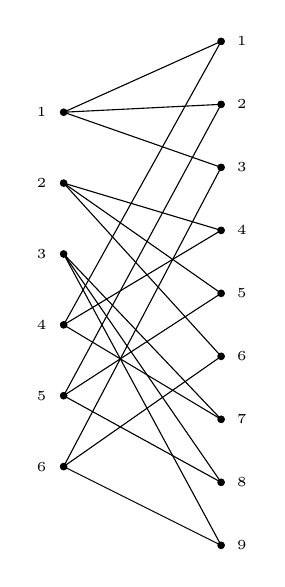
\begin{tikzpicture}[scale=.8]

    \tikzset{type/.style args={[#1]#2}{
        draw,circle,fill,scale=0.25,
        label={[font=\scriptsize, label distance=1pt]#1:#2}
      }}



    \foreach \i in {1,...,6} \draw (0,8-9/8*\i)
    coordinate (Constraint-\i)
    node[type={[180]$\Constraint_\i$}] {};

    \foreach \i in {1,...,9} \draw (2.5,9-\i)
    coordinate (Variable-\i)
    node[type={[0]$\Variable_\i$}] {};

    \foreach \i in {1,...,3} \foreach \j in {1,...,3}
    \pgfmathsetmacro{\k}{(\i-1)*3+\j}
    \draw (Constraint-\i) -- (Variable-\k);

    \foreach \i in {4,...,6} \foreach \j in {1,...,3}
    \pgfmathsetmacro{\k}{\i-3+(\j-1)*3}
    \draw (Constraint-\i) -- (Variable-\k);
  \end{tikzpicture}
  \caption{Type graph $G^\ms$ for the Magic Square game.  }
  \label{fig:type-graph-ms}
\end{figure}

The following theorem records the self-testing (also known as \emph{rigidity})
properties of the Magic Square game.
Its self-testing properties
are crucial to the Pauli basis test.
In particular, it is used to enforce anticommutation relations between certain
pairs of operators.
We will refer to this theorem in the proof of the soundness of the Pauli basis test (\Cref{thm:pauli} below) in \Cref{sec:qld-analysis}.

\begin{theorem}[Rigidity of the Magic Square game]
  \label{thm:ms-rigidity}


Let $\strategy = (\ket{\psi},A,B)$ be a strategy that succeeds in the Magic Square game $\game^{\MS}$ with probability $1 - \eps$, where $\ket{\psi} \in \mH_A \otimes \mH_B$ is a state. Then there exist local isometries $\phi_A: \mH_A \to \mH_{A'} \otimes \mH_{A''},\phi_B: \mH_B \to \mH_{B'} \otimes \mH_{B''}$ (where $\mH_{A'},\mH_{B'} \cong (\C^2)^{\otimes 2}$ and $\mH_{A''},\mH_{B''}$ are finite dimensional) and a state $\ket{\aux} \in \mH_{A''} \otimes \mH_{B''}$ such that 
\begin{enumerate}
    \item $\left \| \phi_A \otimes \phi_B \ket{\psi} - \ket{\EPR_2}^{\otimes 2} \otimes \ket{\aux} \right \| \leq O(\sqrt{\eps})$,
    \item Letting $\tilde{A}^x_a = \phi_A\, A^x_a \, \phi_A^\dagger$ and $\tilde{B}^y_b = \phi_B B^y_b \phi_B^\dagger$, we have that
    \begin{gather*}
        \tilde{A}^{\Variable_1}_b \otimes I_{B'B''} \approx_{\sqrt{\eps}} (\sigma^X_b)_{A'} \otimes I_{A'' B' B''} \\
        \tilde{A}^{\Variable_5}_b \otimes I_{B'B''} \approx_{\sqrt{\eps}} (\sigma^Z_b)_{A'} \otimes I_{A'' B' B''} \\
        I_{A'A''} \otimes \tilde{B}^{\Variable_1}_b    \approx_{\sqrt{\eps}} I_{A' A'' B''} \otimes (\sigma^X_b)_{B'} \\
        I_{A'A''} \otimes \tilde{B}^{\Variable_5}_b    \approx_{\sqrt{\eps}} I_{A' A'' B''} \otimes (\sigma^Z_b)_{B'}
    \end{gather*}
    where the $\approx_{\sqrt{\eps}}$ statement holds with respect to the state $\ket{\EPR_2}^{\otimes 2}_{A'B'} \otimes \ket{\aux}_{A''B''}$ and the answer summation is over $b \in \{0,1\}$. As a consequence, letting 
    \begin{gather*}
    \tilde{A}^{\Variable_1} = \tilde{A}^{\Variable_1}_0 - \tilde{A}^{\Variable_1}_1 \\
    \tilde{A}^{\Variable_5} = \tilde{A}^{\Variable_5}_0 - \tilde{A}^{\Variable_5}_1 \\
    \end{gather*}
    it holds that
    \begin{gather*}
        \tilde{A}^{\Variable_1} \tilde{A}^{\Variable_5} \otimes I_{B' B''} \approx_{\sqrt{\eps}} - \tilde{A}^{\Variable_5}  \tilde{A}^{\Variable_1} \otimes I_{B' B''} \\
        I_{A' A''} \otimes \tilde{B}^{\Variable_1} \tilde{B}^{\Variable_5}  \approx_{\sqrt{\eps}} - I_{A' A''} \otimes \tilde{B}^{\Variable_5}  \tilde{B}^{\Variable_1} \;,
      \end{gather*}
      where the notation $M \approx_{\delta} N$ for $M, N$ that are not POVM
      elements means
      \[  \bra{\psi} (M-N)^\dagger (M-N) \ket{\psi}  \leq  O(\delta). \]
\end{enumerate}

\end{theorem}
\begin{proof}
 	A proof of the rigidity of the Magic Square game can be found in~\cite[Theorem 6.9]{coladangelo2017robust}. There are a couple minor differences between their rigidity statement and the one stated here. First, they state that the robustness of the Magic Square self-test is $O(\eps)$; however they specify the closeness between the actual and ideal states in terms of the trace norm, whereas we specify the closeness between $\phi_\alice \otimes \phi_\bob \ket{\psi}$ and $\ket{\EPR_2}^{\otimes 2}\otimes \ket{\aux}$ in terms of the Euclidean distance, which translates to $O(\sqrt{\eps})$ instead of $O(\eps)$. Second, their choice of ideal strategy specifies that the observables corresponding to $\Variable_1$ and $\Variable_5$ questions are $I \otimes \sigma^Z$ and $\sigma^{Z} \sigma^{X} \otimes \sigma^Z \sigma^X$; however under a local change of basis these are equivalent to $\sigma^X \otimes I$ and $\sigma^Z \otimes I$ respectively.
\end{proof}

We will need the following theorem,
which shows that any pair of anticommuting observables 
can be used to form a value-$1$ strategy for the Magic Square game.

\begin{theorem}
  \label{thm:ms-from-ac}
  Let $A = \{A_b\}_{b \in \F_2}$ and $B = \{B_b\}_{b \in \F_2}$ be two-outcome
  projective measurements acting on $(\C^q)^{\otimes n}$ which are consistent on
  $\ket{\EPR_q}^{\otimes n}$, and let $\mathcal{O}_A = A_0 - A_1$ and
  $\mathcal{O}_B = B_0 - B_1$ be the corresponding observables.
  Suppose that $\mathcal{O}_A \mathcal{O}_B = -\mathcal{O}_B \mathcal{O}_A$.
  Then there exists a symmetric strategy $\strategy = (\psi, M)$ for the Magic
  Square game with the following properties.
  \begin{enumerate}
  \item $\strategy$ is an SPCC strategy of value $1$.
  \item The state $\ket{\psi}$ has the form $\ket{\psi} = \ket{\EPR_q}^{\otimes
      n} \otimes \ket{\EPR_2}$.
  \item For $b \in \{0,1\}$, we have $M^{\Variable_1}_b = A_b \otimes I$ and
    $M^{\Variable_5}_b = B_b \otimes I$.\label{item:embeds}
  \end{enumerate}
\end{theorem}

\begin{proof}
  The strategy~$\strategy$ is based on the canonical two-qubit strategy for the
  Magic Square game as described in, for example,~\cite{aravind2002simple}.
  The state is $\ket{\psi} = \ket{\EPR_q}^{\otimes n} \otimes \ket{\EPR_2}$.
  We specify the measurements of~$\strategy$ in
  Figure~\ref{fig:ms-operator-soln} as an \emph{operator solution} for the Magic
  Square game, meant to be read as follows: each cell contains a two-outcome
  projective measurement $\{E_0, E_1\}$ on $(\C^q)^{\otimes n} \otimes \C^2$
  written as its \emph{$\pm 1$-valued observable} $E_0 - E_1$.
  When Player~$\alice$ or~$\bob$ receives the question $\Variable_j$ for $j \in
  \{1, \ldots, 9\}$, they measure their share of~$\ket{\psi}$ using the
  measurement specified by the cell corresponding to~$\Variable_j$ and receive a
  single-bit measurement.
  When they receive the question $\Constraint_i$ for $i \in \{1,2,\ldots,6\}$,
  they simultaneously perform the three measurements in the corresponding row or
  column on $\ket{\psi}$ to obtain three bits.
  For example, if Player~$\alice$ receives question~$\Variable_1$, they
  measure~$\ket{\psi}$ using the measurement $\{A_0 \otimes I, A_1 \otimes I\}$
  corresponding to the observable $\cal{O}_A \otimes I$ (where the first
  operator acts on $\ket{\EPR_q}^{\otimes n}$ and the second acts on
  $\ket{\EPR_2}$).
  Similarly, on question~$\Variable_5$, they use the measurement $\{B_0 \otimes
  I, B_1 \otimes I\}$.
  This establishes Item~\ref{item:embeds} of the theorem.
  \begin{figure}[ht!]
    \begin{center}
      \renewcommand{\arraystretch}{2.4}
      \begin{tabularx}{.6\textwidth}{| X | X | X |}
        \hline
        $ \phantom{I\;\;O}\cal{O}_A\, \otimes \; \;I$
        & $ \phantom{\cal{O}_BO} I\;\;\, \otimes \; \sigma^X$
        & $ \phantom{\cal{O}_B\;}\cal{O}_A\, \otimes \; \sigma^X$ \\
        \hline
        $ \phantom{\cal{O}_AO} I\;\;\, \otimes \; \sigma^Z$
        & $ \phantom{I\;\;O}\cal{O}_B\, \otimes \; \;I$
        & $ \phantom{\cal{O}_A\;}\cal{O}_B\, \otimes \; \sigma^Z$ \\
        \hline
        $ \phantom{I\;\;O}\cal{O}_A \, \otimes \; \sigma^Z$
        & $ \phantom{I\;\;O}\cal{O}_B \, \otimes \; \sigma^X$
        & $ \; \cal{O}_A \cal{O}_B \, \otimes \; \sigma^Z \sigma^X$ \\
        \hline
      \end{tabularx}
      \caption{Observables for Magic Square strategy}
      \label{fig:ms-operator-soln}
		\end{center}
  \end{figure}
  
  First, we show that this gives a well-defined strategy.
  The $\Variable_j$ measurements are well-defined because each cell contains a
  $\pm 1$-valued observable.
  This is obvious for all $j \neq 9$; when $j = 9$, the bottom-right cell
  contains $\cal{O}_A \cal{O}_B \otimes \sigma^Z \sigma^X$.
  Because~$\cal{O}_A$ and~$\cal{O}_B$ anti-commute,
  \begin{equation}\label{eq:am-i-hermitian}
  \cal{O}_A \cal{O}_B \otimes \sigma^Z \sigma^X
  = - \cal{O}_A \cal{O}_B \otimes \sigma^X \sigma^Z
  = \cal{O}_B \cal{O}_A \otimes \sigma^X \sigma^Z
  = (\cal{O}_A \cal{O}_B \otimes \sigma^Z \sigma^X)^\dagger.
  \end{equation}
  As a result, this matrix is Hermitian. In addition, 
  \begin{equation*}
  (\cal{O}_A \cal{O}_B \otimes \sigma^Z \sigma^X)^2
  = (\cal{O}_A \cal{O}_B \otimes \sigma^Z \sigma^X) \cdot (\cal{O}_B \cal{O}_A \otimes \sigma^X \sigma^Z)
  = (\cal{O}_A \cal{O}_B \cdot \cal{O}_B \cal{O}_A) \otimes (\sigma^Z \sigma^X \cdot \sigma^X \sigma^Z)
  = I,
  \end{equation*}
  where the first step uses Equation~\eqref{eq:am-i-hermitian} and the final
  step uses the fact that $\cal{O}_A, \cal{O}_B, \sigma^X, \sigma^Z$ are $\pm
  1$-valued observables and hence square to the identity.
  As a result, this matrix is Hermitian and squares to the identity.
  Therefore, it is a $\pm 1$-valued observable.
  
  As for the $\Constraint_i$ measurements,
  we must show that the three measurements in each row and column are simultaneously measurable.
  This is equivalent to the three $\pm 1$-valued observables being simultaneously diagonalizable,
  which is equivalent to them being pairwise commuting. This can be easily verified for the cases of $i = 1, 2, 4, 5$
  (i.e.\ the first two rows and columns).
  In the case of $i = 3$, commutativity of $\cal{O}_A \otimes \sigma^Z$ and $\cal{O}_B \otimes \sigma^X$ 
  follows from Equation~\eqref{eq:am-i-hermitian}.
  Since these two matrices commute, they also commute with their product 
  $(\cal{O}_A \otimes \sigma^Z)(\cal{O}_B \otimes \sigma^X) = \cal{O}_A \cal{O}_B \otimes \sigma^Z \sigma^X$.
  The case of $i = 6$ is similar.
  
  By construction, $\strategy$ is symmetric, and we have already shown that it
  is projective.
  It remains to show that it is commuting, consistent, and value~$1$.
  To show that it is commuting, it suffices to show that the measurement for
  each cell is simultaneously measurable with all three measurements in its row
  or column, which was already proved above.
  Now we show consistency of the measurements.
  We will show this by instead showing consistency of their observables.
  By this we mean the following: if $E = \{E_0, E_1\}$ is a two-outcome projective measurement on $\cal{H}$
  then its corresponding $\pm 1$-valued observable $\cal{O} = E_0 - E_1$
  is consistent on a state $\ket{\phi} \in \cal{H} \otimes \cal{H}$ if
  \begin{equation*}
  \cal{O}\otimes I_{\bob} \cdot \ket{\phi} = I_{\alice} \otimes \cal{O} \cdot \ket{\phi}.
  \end{equation*}
  This is in fact equivalent to the notion of $E$ being consistent on $\ket{\phi}$ from Definition~\ref{def:consistent-measurement}.
  To see this, if $E$ is consistent on $\ket{\phi}$, then so is $\cal{O}$, because
  \begin{equation*}
  \cal{O}\otimes I_{\bob} \cdot \ket{\phi}
  = (E_0 - E_1) \otimes I_{\bob} \cdot \ket{\phi}
  = I_{\alice} \otimes (E_0 - E_1) \cdot \ket{\phi}
  = I_{\alice} \otimes \cal{O} \cdot \ket{\phi},
  \end{equation*}
  where the second equality is by consistency of~$E$.
  On the other hand, suppose $\cal{O}$ is consistent on $\ket{\phi}$.
  Then because $E_0 + E_1 = I$, we can write $E_0 = \tfrac{1}{2} \cdot (I + \cal{O})$ and $E_1 = \tfrac{1}{2} \cdot (I - \cal{O})$.
  As a result,
  \begin{equation*}
  E_0 \otimes I_{\bob} \cdot \ket{\phi}
  = \tfrac{1}{2} \cdot (I + \cal{O}) \otimes I_{\bob} \cdot \ket{\phi}
  = I_{\alice} \otimes \tfrac{1}{2} \cdot (I + \cal{O}) \cdot \ket{\phi}
  = I_{\alice} \otimes E_0 \cdot \ket{\phi},
  \end{equation*}
  and similarly for $E_0$. Thus, $E$ is consistent on $\ket{\phi}$.
  This proves the equivalence.
  
  Now we use this to prove consistency of $\strategy$.
  To begin, we note that because $A$ and $B$ are consistent on $\ket{\EPR_q}^{\otimes n}$ by assumption,
  so to are their $\pm 1$-valued observables $\cal{O}_A$ and $\cal{O}_B$.
  Next, we note that $\sigma^X$ and $\sigma^Z$ are consistent on $\ket{\mathrm{EPR}_2}$;
  to verify this, we recall that $\sigma^X \ket{0} = \ket{1}$ and $\sigma^X \ket{1} = \ket{0}$, and so
  \begin{align*}
  \sigma^X \otimes I_{\bob} \cdot \ket{\mathrm{EPR}_2}
&  =   \sigma^X \otimes I_{\bob} \cdot \tfrac{1}{\sqrt{2}} (\ket{00} + \ket{11})\\
&  = \tfrac{1}{\sqrt{2}} (\ket{10} + \ket{01})
    =    I_{\alice} \otimes \sigma^X \cdot \tfrac{1}{\sqrt{2}} (\ket{11} + \ket{00})
    =    I_{\alice} \otimes \sigma^X \cdot \ket{\mathrm{EPR}_2}.
  \end{align*}
  This shows $\sigma^X$ is consistent on $\ket{\mathrm{EPR}_2}$,
  and a similar argument shows the same for $\sigma^Z$.
  We now use these two facts to show that the observable in each cell of
  Figure~\ref{fig:ms-operator-soln} is consistent on $\ket{\psi}$.
  To see why, consider the $j = 9$ case:
  \begin{align*}
&  (\cal{O}_A \cal{O}_B \otimes \sigma^Z \sigma^X)_\alice \otimes I_\bob
		\cdot \ket{\EPR_q}^{\otimes n} \otimes \ket{\EPR_2} \\
  ={}& (\cal{O}_A \cal{O}_B \otimes \sigma^Z)_\alice \otimes (I \otimes \sigma^X)_\bob
  		\cdot \ket{\EPR_q}^{\otimes n} \otimes \ket{\EPR_2}\tag{consistency of $\sigma^X$}\\
  ={}& (\cal{O}_A \cal{O}_B \otimes I)_\alice \otimes (I \otimes \sigma^X\sigma^Z)_\bob
  		\cdot \ket{\EPR_q}^{\otimes n} \otimes \ket{\EPR_2}\tag{consistency of $\sigma^Z$}\\
  ={}& (\cal{O}_A \otimes I)_\alice \otimes ( \cal{O}_B \otimes \sigma^X\sigma^Z)_\bob
  		\cdot \ket{\EPR_q}^{\otimes n} \otimes \ket{\EPR_2}\tag{consistency of $\cal{O}_B$}\\
  ={}& I_\alice \otimes (\cal{O}_B \cal{O}_A \otimes \sigma^X\sigma^Z)_\bob
  		\cdot \ket{\EPR_q}^{\otimes n} \otimes \ket{\EPR_2}\tag{consistency of $\cal{O}_A$}\\
  ={}& I_\alice \otimes (\cal{O}_A \cal{O}_B \otimes \sigma^Z \sigma^X)_\bob
  		\cdot \ket{\EPR_q}^{\otimes n} \otimes \ket{\EPR_2}. \tag{by Equation~\eqref{eq:am-i-hermitian}}
  \end{align*}
  The remaining cases of $j \in\{1, \ldots, 8\}$ are similar, and we omit them.
  This shows that the observable in each cell is consistent on $\ket{\psi}$,
  and as a result the corresponding two-outcome projective measurements are consistent as well.
  As a result, the $\Variable_j$ measurements are consistent.
  
  As for the $\Constraint_i$ measurements, each such measurement $\{F_{a, b,
    c}\}_{a, b, c \in \{0, 1\}}$ is of the form $F_{a, b, c} = E^1_a \cdot E^2_b
  \cdot E^3_c$, where $E^1$, $E^2$, and $E^3$ are $\Variable$ measurements.
  But then consistency of~$F$ follows from the~$\Variable$ consistencies:
  \begin{align*}
  F_{a, b, c} \otimes I_{\bob} \ket{\psi}
 & = (E^1_a \cdot E^2_b \cdot E^3_c)_{\alice} \otimes I_{\bob} \ket{\psi}\\
 & = (E^1_a \cdot E^2_b)_{\alice} \otimes (E^3_c)_{\bob} \ket{\psi} \tag{consistency of $E^3$}\\
 &   = (E^1_a)_{\alice} \otimes (E^3_c \cdot E^2_b)_{\bob} \ket{\psi}\tag{consistency of $E^2$}\\
 &       = I_{\alice} \otimes (E^3_c \cdot E^2_b \cdot E^1_a)_{\bob} \ket{\psi}\tag{consistency of $E^1$}\\
 &       = I_{\alice} \otimes (E^1_a \cdot E^2_b \cdot E^2_c)_{\bob} \ket{\psi}\tag{commutativity of $E^1$, $E^2$, and $E^3$}\\
 &               = I_{\alice} \otimes F_{a, b,c} \ket{\psi}.
  \end{align*}
  Hence, all measurements are consistent.
  
  Since all measurements are consistent, this implies that the answer bit of the
  player receiving a $\Variable$ question is always consistent with the
  corresponding answer bit of the player receiving the $\Constraint$ question.
  Similarly, the answers of the player receiving the $\Constraint$ question
  always satisfy the given constraint; observe that in all rows and the first
  two columns, the observables multiply to $I$, whereas the observables in the
  last column multiply to $-I$.
  This implies that the strategy is value-$1$.
  To see why, 
  let us again consider a $\Constraint_i$ measurement, which we write as $F=\{F_{a, b, c}\}_{a, b, c \in \{0, 1\}}$.
  As above, it can be written as  $F_{a, b, c} = E^1_a \cdot E^2_b \cdot E^3_c$, where $E^1$, $E^2$, and $E^3$ are $\Variable$ measurements.
  Consider the measurement $S=\{S_0, S_1\}$ that corresponds to measuring $\{F_{a, b, c}\}$ and then outputting the sum of measured values of~$a$, $b$, and~$c$.
  In other words,
  \begin{equation*}
  S_0 = F_{0, 0, 0} + F_{0, 1, 1} + F_{1, 0, 1} + F_{1, 1, 0},
  \qquad
  S_1 = F_{0, 0, 1} + F_{0, 1, 0} + F_{1, 0, 0} + F_{1, 1, 1}.
  \end{equation*}
  The following expression gives a convenient formula for the $\pm 1$-valued observable $S_0 - S_1$:
  \begin{equation*}
  (E_0^1 - E_1^1) \cdot (E_0^2 - E_1^2) \cdot (E_0^3 - E_1^3)
  = E_0^1 E_0^2 E_0^3 - E_0^1 E_0^2 E_1^3 - E_0^1 E_1^2 E_0^3 + E_0^1 E_1^2 E_1^3 + \cdots
  = S_0 - S_1.
  \end{equation*}
  When we are looking at $\Constraint_i$ for $i \in \{1, 2, 3, 4, 5\}$,
  the left-hand side of this equation is equal to $I$, and so $I = S_0- S_1$.
  Because $S_0$ and $S_1$ are both positive semidefinite,
  this is true only if $S_0 = I$ and $S_1 = 0$, which implies that the three bits output by $F$ always sum to~$0$.
  As a result, this strategy always satisfies the $\Constraint_i$ question.
  On the other hand, when $i = 6$, then the left-hand side of this equation is equal to $-I$,
  and so $S_1 = I$, and the three bits sum to~$1$.
  Thus, the strategy always satisfies the $\Constraint_6$ question as well.
  This concludes the proof.
\end{proof}

\subsection{The Pauli basis test}
\label{sec:pauli-verifier}

We introduce the quantum low-degree test of~\cite{natarajan2018low} in the form
of a slight modification to it by~\cite{NW19} known as the \emph{Pauli basis
  test}.
Informally, the quantum low-degree test asks the players to measure a large
number of qubits and return a highly compressed version of the measurement
outcome.
The Pauli basis test simply asks that the players return their uncompressed
measurement outcomes, and it is designed by direct reduction to the quantum
low-degree test.
In Section~\ref{sec:qld-game} we describe the Pauli basis test as a nonlocal
game $\game^\pauli$ and show that its question distribution is implementable via
a CL distribution, as we did with the classical low-degree test in
Section~\ref{sec:ld-verifier}.
In Section~\ref{sec:qld-complexity} we exhibit canonical parameters for the
Pauli basis test and give bounds on the time complexity of executing the test.

\subsubsection{The game}
\label{sec:qld-game}

We start by discussing parameter settings.
The game $\game^\pauli$ is parametrized by a tuple
\[\qldparams = (q,m,d)\;,\] where $q,m,d \in \N$ are integers. 
We sometimes write $\game^\pauli_\qldparams$ to emphasize the dependence of the
Pauli basis test on the parameters.

Informally, the test is meant to certify that the players share a state of the
form $\ket{\EPR_q}^{\otimes M}$, where $M=2^m$.
Its question set includes questions that are axis-parallel/diagonal lines and points in $\F_q^m$,
which are meant to correspond to questions in the classical low-degree test, and questions
of the form $(\Pauli, W)$, for $W \in \{X, Z\}$.
Upon receipt of a question of the latter form, the players are expected to
perform the POVM $\{\tau_h^W\}_{h \in \F_q^{M}}$ and report the outcome $h$ as
their answer.

The key idea behind the test
is for the provers to encode their outcomes using the \emph{low-degree encoding} from Section~\ref{sec:ld-encoding}.
Given an outcome $h \in \F_q^M$, the low-degree encoding of~$h$ is the polynomial $g_h:\F_q^m \rightarrow \F_q$.
Rather than asking the provers to always return the entire string~$h$,
many of the subtests in the game $\game^\pauli$ will ``probe'' limited information about~$h$ as follows:
the verifier provides the provers with a string $u_W \in \F_q^m$,
and using this they are expected to evaluate $g_h(u_W) \in \F_q$ and return it to the verifier.
For a fixed value of~$W$, then, the prover's responses to these ``probes'' should be consistent with some low-degree polynomial in the input~$u_W$.
To check this, the verifier can perform the classical low-degree test from Section~\ref{sec:ld-verifier}.
This ensures that the prover's responses for the $W = X$ basis are consistent with each other,
as well as their responses for the $W = Z$ basis, although it does not test consistency between the $X$ and $Z$ responses.

The next set of subtests the verifier performs ensure that the provers' $X$ and $Z$ measurements are consistent with each other.
On the $X$ side, consider the measurement in which the prover performs the $\{\tau_h^X\}$ POVM,
receives outcome $h_X$, and outputs $g_{h_X}(u_X) \in \F_q$.
For technical reasons that will become clear shortly,
it will be convenient for the prover's measurement to have two outcomes rather than~$q$ outcomes.
To accomplish this, the verifier also provides the prover with an element $r_X \in \F_q$;
given this, the prover should output not $g_{h_X}(u_X) \in \F_q$ but $\tr(g_{h_X}(u_X) \cdot r_X)$, which is an element of $\F_2$.
Similarly, on the $Z$ side, suppose the prover is provided $r_Z \in \F_q$,
performs $\{\tau_h^Z\}$ to receive $h_Z$, and outputs $\tr(g_{h_Z}(u_Z) \cdot r_Z) \in \F_2$.
Together, these two are a pair of two-outcome measurements, one in the~$X$ basis and one in the~$Z$ basis,
and as it turns out, this pair of measurements either commutes with each other or anticommutes with each other
(this is why we modified the measurements to have only two outcomes).
The key quantity to determine which of these is the case is the following complicated-looking expression:
\begin{equation*}
\gamma = \tr \bigl( (\ind_{m}(u_\xpt) \cdot r_\xpt) \cdot
      (\ind_{m}(u_\zpt) \cdot r_\zpt) \bigr)\;.
\end{equation*}
If $\gamma = 0$, then these two measurements commute, and if $\gamma = 1$, then these two measurements anticommute
(this fact is established in the proof of Lemma~\ref{lem:pauli-completeness} below).
In the $\gamma = 0$ case, the verifier can check whether these two measurements commute by performing the ``commutation check'',
which asks the provers to simultaneously measure both $\tr(g_{h_X}(u_X) \cdot r_X)$ and $\tr(g_{h_Z}(u_Z) \cdot r_Z)$ and report their values.
In the $\gamma = 1$ case, on the other hand, the measurements anticommute, which implies that they cannot simultaneously be measured.
In spite of this, the verifier can still check that the measurements anticommute by using the Magic Square game from Section~\ref{sec:ms} above.
As was shown in Theorem~\ref{thm:ms-from-ac}, any pair of anticommuting measurements
can be used to form a perfect strategy for the Magic Square game
(and indeed the reverse is true as well: any perfect strategy for the Magic Square game entails a pair of anticommuting measurements).

Together, these give the main subtests for the game $\game^\pauli$.

\begin{definition}[Admissible parameters]\label{def:admissible}
  We say that the tuple $\qldparams=(q, m, d)$ is \emph{admissible} if $q$ is
  an admissible field size (Definition~\ref{def:admissible-size}) and $m | q$.
\end{definition}


\paragraph{Question distribution.}
We now describe the question distribution of the game $\game^\pauli$, and show
that it is a (typed) CL distribution.
The question types in the game $\game^\pauli$ are
\begin{equation}
  \label{eq:pauli-type}
  \type^\pauli= \bigl( \{\Point, \ALine, \DLine, \Pauli, \Pair \} \times \{X,Z\} \bigr)
  \cup \type^\ms \cup \{\Pair\}\;,
\end{equation}
where $\type^\ms$ is the question type set of the Magic Square game defined in
Section~\ref{sec:ms}.




Before presenting the CL functions of the Pauli basis test, we first give an
intuitive description of the question distribution of the Pauli basis test: a
pair of questions $((\tvar_\alice, x_\alice), (\tvar_\bob, x_\bob))$ in
$\game^\pauli$ can be sampled via the following procedure:

\begin{enumerate}
\item Sample a pair of types by sampling an edge $(\tvar_\alice, \tvar_\bob)$ of
  the graph $G^\pauli$ given in Figure~\ref{fig:type-graph-pauli} uniformly at
  random (including the self-loops).
\item Sample the following uniformly at random:
	\begin{enumerate}
	\item (\emph{Points}) $u_\xpt,u_\zpt \in \F_q^m$,
	\item (\emph{Directions}) $s \in \F_q$, $v \in \F_q^m$,
  \item (\emph{Qubit basis for (anti-)commutation}) $r_\xpt,r_\zpt \in \F_q$.
	\end{enumerate}
\item For $w \in \AB$ and $W\in\{X,Z\}$,
	\begin{enumerate}
  \item If $\tvar_w = (\Point, W)$, then set $x_w = u_W$,
  \item If $\tvar_w = (\ALine, W)$, then set $x_w = (u_0,s)$, where $u_0 =
    L^\lnf_{e_i}(u_W)$, with $i = \chi(s)$ (see \Cref{sec:ld-game} for
    definition of $L^\lnf$ and $\chi(s)$),
  \item If $\tvar_w = (\DLine,W)$, then set $x_w = (u_0,s,v')$, where $i =
    \chi(s)$, $v' = \pi_{i-1}(v)$, and $u_0 = L^\lnf_{v'}(u_W)$,
  \item If $\tvar_w = \Constraint_i$ for some $i\in\{1,\ldots,6\}$, then set
    $x_w = (u_\xpt, u_\zpt, r_\xpt, r_\zpt)$,
  \item If $\tvar_w = \Variable_j$ for some $j\in\{1,\ldots,9\}$, then set $x_w
    = (u_\xpt, u_\zpt, r_\xpt, r_\zpt)$,
  \item If $\tvar_w = \Pair$, then set $x_w = (u_\xpt, u_\zpt, r_\xpt, r_\zpt)$,
  \item If $\tvar_w = (\Pair, W)$, then set $x_w = (u_\xpt, u_\zpt, r_\xpt, r_\zpt)$,
  \item If $\tvar_w = (\Pauli, W)$, then set $x_w = 0$.
	\end{enumerate}
\end{enumerate}

\begin{figure}[!htbp]
  \centering
  \begin{tikzpicture}[scale=.8]

    \tikzset{type/.style args={[#1]#2}{
        draw,circle,fill,scale=0.25,
        label={[font=\scriptsize, label distance=1pt]#1:#2}
      }}



    \foreach \i in {1,...,6} \draw (0,8-9/8*\i)
    coordinate (Constraint-\i)
    node[type={[180]$\Constraint_\i$}] {};

    \foreach \i in {1,...,9} \draw (2.5,9-\i)
    coordinate (Variable-\i)
    node[type={[330]$\Variable_\i$}] {};

    \foreach \i in {1,...,3} \foreach \j in {1,...,3}
    \pgfmathsetmacro{\k}{(\i-1)*3+\j}
    \draw (Constraint-\i) -- (Variable-\k);

    \foreach \i in {4,...,6} \foreach \j in {1,...,3}
    \pgfmathsetmacro{\k}{\i-3+(\j-1)*3}
    \draw (Constraint-\i) -- (Variable-\k);



  	\draw (6,9) coordinate (DLine-X) node[type={[90]$(\DLine, X)$}] {};
    \draw (8,9) coordinate (ALine-X) node[type={[90]$(\ALine, X)$}] {};
    \draw (7,8) coordinate (Point-X) node[type={[315]$(\Point, X)$}] {};
    \draw (9.5,8) coordinate (Pauli-X) node[type={[0]$(\Pauli, X)$}] {};
    \draw (6,3) coordinate (DLine-Z) node[type={[270]$(\DLine, Z)$}] {};
    \draw (8,3) coordinate (ALine-Z) node[type={[270]$(\ALine, Z)$}] {};
    \draw (7,4) coordinate (Point-Z) node[type={[45]$(\Point, Z)$}] {};
    \draw (9.5,4) coordinate (Pauli-Z) node[type={[0]$(\Pauli, Z)$}] {};
    \draw (8,6) coordinate (Pair) node[type={[0]$\Pair$}] {};
    \draw (7.3,6.8) coordinate (Pair-X) node[type={[0]$(\Pair,X)$}] {};
    \draw (7.3,5.2) coordinate (Pair-Z) node[type={[0]$(\Pair,Z)$}] {};



    \foreach \from/\to in {ALine-X/Point-X, DLine-X/Point-X, Point-X/Pauli-X,
      DLine-Z/Point-Z, ALine-Z/Point-Z, Point-Z/Pauli-Z,
      Point-X/Variable-1, Point-Z/Variable-5}
    \draw (\from) -- (\to);

    \draw (Point-X) to [out=275,in=120] (Pair-X) to [out=300,in=140] (Pair);
    \draw (Point-Z) to [out=85,in=240] (Pair-Z) to [out=60,in=220] (Pair);

  \end{tikzpicture}
  \caption{Graph $G^\pauli$ for the Pauli basis test.
    Each vertex also has a self-loop which is not drawn on the figure for
    clarity.}
  \label{fig:type-graph-pauli}
\end{figure}

We now specify the corresponding CL functions for each of the question types in
the Pauli basis test.

\paragraph{Conditional linear functions for the Pauli basis test.}
The CL functions corresponding to the Pauli basis test question distribution are
parameterized by the parameter tuple $\qldparams = (q,m,d)$.
Let $V^\pauli$ denote the linear space $(\F_q^m)^2 \times \F_q \times \F_q^m
\times (\F_q)^2$.
The space $V^\pauli$ is decomposed into a direct sum of the following register
subspaces: $V_\xpt,V_\zpt$ (which are $m$-dimensional), $V_\coord$ (which is
$1$-dimensional), $V_{\dir{}}$ (which is $m$-dimensional), and
$V_{\rxpt},V_{\rzpt}$ (which are $1$-dimensional).
We identify elements of $V^\pauli$ as tuples $(u_\xpt,u_\zpt,s,v,r_\xpt,r_\zpt)
\in (\F_q^m)^2 \times \F_q \times \F_q^m \times (\F_q)^2$.
We define CL functions $L_\tvar: V^\pauli \to V^\pauli$ for every type $\tvar
\in \type^\pauli$:
\begin{enumerate}
\item For $W \in \{X,Z\}$, define $L_{\Point,W}(u_\xpt,u_\zpt,s,v,r_\xpt,r_\zpt)
  = L_\Point(u_W,s,v)$ where $L_\Point$ is the $1$-level CL function defined in
  \Cref{eq:cl-ptf}.\footnote{The range $V_{\xpt} \oplus V_\coord \oplus
    V_{\dir{}}$ or $V_{\zpt} \oplus V_\coord \oplus V_{\dir{}}$ of $L_\Point$ is
    embedded in $V^\pauli$ in the natural way.
    The same convention is used also in Item 2 and 3 for $L_\ALine$ and
    $L_\DLine$.}
\item For $W \in \{X,Z\}$, define $L_{\ALine,W}(u_\xpt,u_\zpt,s,v,r_\xpt,r_\zpt)
  = L_\ALine(u_W,s,v)$ where $L_\ALine$ is the $2$-level CL function defined in
  \Cref{eq:cl-alnf}.
\item For $W \in \{X,Z\}$, define $L_{\DLine,W}(u_\xpt,u_\zpt,s,v,r_\xpt,r_\zpt)
  = L_\DLine(u_W,s,v)$ where $L_\DLine$ is the $3$-level CL function defined in
  \Cref{eq:cl-dlnf}.
\item For $\tvar \in \type^\ms \cup \{\Pair, (\Pair,X), (\Pair,Z) \}$,
  $L_{\tvar}(u_\xpt,u_\zpt,s,v,r_\xpt,r_\zpt) =
  (u_\xpt,u_\zpt,0,0,r_\xpt,r_\zpt)$, i.e., it projects onto $V_\xpt \oplus
  V_\zpt \oplus V_{\rxpt} \oplus V_{\rzpt}$.
  Thus $L_{\tvar}$ is a $1$-level CL function.
  
\item For $W \in \{X,Z\}$, define $L_{\Pauli,W} = 0$ as the identically $0$
  function.
  Thus it is a $0$-level CL function.

\end{enumerate}
We note that the maps $L_{\Point,W}, L_{\ALine,W}, L_{\DLine,W}$ act as the zero function
on $V_{\overline{W}} \oplus V_{\rxpt} \oplus V_{\rzpt}$ where $\overline{W} = X$
if $W = Z$ and $\overline{W} = Z$ if $W = X$.

The question distribution of $\game^\pauli$ is thus a typed CL distribution on
$\type^\pauli \times V^\pauli \times \type^\pauli \times V^\pauli$ where
$(\tvar_\alice,x_\alice,\tvar_\bob,x_\bob)$ is sampled by first uniformly
sampling an edge $(\tvar_\alice,\tvar_\bob)$ from the graph $G^\pauli$ defined
in Figure~\ref{fig:type-graph-pauli}, sampling a uniformly random $z \in
V^\pauli$, and then setting $x_w = L_{\tvar_w}(z)$ for $w \in \AB$.





\paragraph{Decision procedure.}
The decision procedure for $\game^\pauli$ is presented in
Figure~\ref{fig:decider_pauli}.
Similarly to Figure~\ref{fig:ld-decider}, we provide a table that summarizes a
parsing scheme for the questions and answers, depending on the type of question.
The answers are bit strings that are interpreted as more structured objects such
as elements over $\F_q$, vectors, or polynomials, depending on the question.
In the ``low-degree check'', the decision procedure $\decider^\pauli$ calls the
classical low-degree decision procedure $\decider^\ld$ parametrized by the tuple
$\ldparams = (q,m,d,1)$ (defined in Section~\ref{sec:ld-verifier}) as a
subroutine.


\begin{figure}[H]
  \begin{gamespec}
    \vspace{9pt}
    \begin{center}
      \renewcommand\arraystretch{1.3}
      \begin{tabularx}{.92\textwidth}{ l X l }
        \toprule
        Type & Question Content & Answer Format \\
        \midrule
        (\Point, $W$) & $y \in  \F_q^m$ & Element of $\F_q$  \\
        (\ALine, $W$) & $(u_W, s) \in \F_q^m \times \F_q$
        & Polynomial $f: \F_q \to \F_q$\\
        (\DLine, $W$) & $(u_W, s, v) \in \F_q^m \times \F_q \times \F_q^m$ 
        & Polynomial $f: \F_q \to \F_q$ \\
        \Pair & $(u_\xpt, u_\zpt, r_\xpt, r_\zpt) \in
        (\F_q^m)^2 \times \F_q^2 $ & $(\beta_\xpt,\beta_\zpt) \in \F_2^2$ \\
        (\Pair, $W$) & $(u_\xpt, u_\zpt, r_\xpt, r_\zpt) \in
        (\F_q^m)^2 \times \F_q^2 $ & Element of $\F_2$ \\
        $\Constraint_i$ & $(u_\xpt, u_\zpt, r_\xpt, r_\zpt) \in (\F_q^m)^2
        \times \F_q^2$ &
        $(\alpha_{v_1}, \alpha_{v_2}, \alpha_{v_3}) \in \F_2^3$ \\
        $\Variable_j$ & $(u_\xpt, u_\zpt, r_\xpt, r_\zpt) \in
        (\F_q^m)^2 \times \F_q^2$ & Element of $\F_2$ \\
        (\Pauli, $W$) & $0$ & Element of $\F_q^{M}$ \\
        \bottomrule \multicolumn{3}{c}{Table: Question and answer format of the
          Pauli basis game.}
      \end{tabularx}
    \end{center}
    \vspace{9pt}

    On input $(\tvar_\alice,x_\alice, \tvar_\bob, x_\bob, a_\alice, a_\bob)$,
    the decision procedure $\decider^\pauli$ performs the following checks for
    $w \in \AB$:
    \begin{enumerate}[itemsep=2pt,parsep=2pt]
    \item (\textbf{Consistency check}).
      \label{item:same-type}
      If $\tvar_\alice = \tvar_\bob$, accept iff $a_\alice = a_\bob$.

    \item (\textbf{Low-degree}).
      \label{item:low-degree}
      Let $\ldparams = (q,m,d,1)$. 
      \begin{enumerate}
      	\item If $\tvar_w = (\Point, W), \tvar_{\overline{w}} = (\ALine, W)$, accept if
      $\decider^\ld_{\ldparams}$ accepts $(\Point, x_w, \ALine, x_{\overline{w}}, a_w,
      a_{\overline{w}})$.
      	\item If $\tvar_w = (\Point, W), \tvar_{\overline{w}} = (\DLine, W)$, accept if
      $\decider^\ld_{\ldparams}$ accepts $(\Point, x_w, \DLine, x_{\overline{w}}, a_w,
      a_{\overline{w}})$.
		\end{enumerate}
    \item (\textbf{Consistency check}).
      \label{item:low-degree-consistency}
      If $\tvar_w = (\Point, W), \tvar_{\overline{w}} = (\Pauli, W)$, accept if
      $g_{a_{\overline{w}}}(x_w) = a_w$, where $g_{a_{\overline{w}}}$ is
      the low-degree encoding of $a_{\overline{w}} \in \F_q^M$ defined in
      Section~\ref{sec:ld-encoding}.
    \end{enumerate}
    In the remaining four cases, the decision procedure first computes the
    number
    \begin{equation}
      \label{eq:gamma-value}
      \gamma = \tr \bigl( (\ind_{m}(u_\xpt) \cdot r_\xpt) \cdot
      (\ind_{m}(u_\zpt) \cdot r_\zpt) \bigr)\;,
    \end{equation}
    where we recall the $\ind_{m}(\cdot)$ vector from Section~\ref{sec:ld-encoding}.
    \begin{enumerate}[itemsep=2pt,parsep=2pt]
      \setcounter{enumi}{3}
    \item (\textbf{Commutation check}).
      \label{item:commutation} If $\tvar_w = (\Pair, W), \tvar_{\overline{w}} =
      \Pair$, accept if $a_w = \beta_W$ or $\gamma \neq 0$.
    \item (\textbf{Consistency check}).
      \label{item:commutation-consistency} If $\tvar_w = (\Point,W), \tvar_{\overline{w}} =
      (\Pair,W)$, accept if $\tr (a_w r_W) = a_{\overline{w}}$ or $\gamma \neq 0$.
      
    \item (\textbf{Magic square check}).
      \label{item:magic-square} If $\tvar_w = \Constraint_i,
      \tvar_{\overline{w}} = \Variable_j$, accept if $\gamma = 0$, or $a_w$
      satisfies constraint $\Constraint_i$ and $ \alpha_j = a_{\overline{w}}$.

    \item (\textbf{Consistency check}).
      \label{item:magic-square-consistency}
      If $\tvar_w = (\Point,W), \tvar_{\overline{w}} = \Variable_j$, accept if
      $\gamma = 0$ or if $j = 1$, $W = X$, and $\tr(a_w r_\xpt) =
      a_{\overline{w}}$ or if $j = 5$, $W = Z$, and $\tr(a_w r_\zpt) =
      a_{\overline{w}}$.
    \end{enumerate}
  \end{gamespec}
  \caption{Specification of the decision procedure $\decider^\pauli_\qldparams$.}
  \label{fig:decider_pauli}
\end{figure}

We describe an honest, value-$1$ PCC strategy for the Pauli basis test.


\begin{lemma}\label{lem:pauli-completeness}
  The Pauli basis test $\game^\pauli_\qldparams$ has a value-$1$ SPCC strategy.
\end{lemma}

\begin{proof}
  We begin by specifying the value-$1$ strategy $\strategy = (\ket{\psi}, E)$.
  The state is
  \begin{equation*}
    \ket{\psi} = \ket{\EPR_q}^{\otimes M} \otimes \ket{\EPR_2}\;.
  \end{equation*}
  Now we specify the measurements.
  We start with measurements associated with questions of type $\Point$,
  $\ALine$, $\DLine$, and $\Pauli$.
  Using notation introduced in Section~\ref{sec:ld-encoding}, for $W \in \{X,
  Z\}$,
  \begin{align*}
    E^{(\Point,W),\, y}_{\, a}
    & = \tau^W_{[g_{\cdot}(y) = a]} \otimes I\;,\\
    E^{(\ALine,W),\, \line}_{\, f}
    & = \tau^W_{[(g_{\cdot})|_\line = f]} \otimes I\;,\\
    E^{(\DLine,W),\, \line}_{\, f}
    & = \tau^W_{[(g_{\cdot})|_\line = f]} \otimes I\;,\\    
    E^{(\Pauli,W)}_{\, a}
    & = \tau^W_{a} \otimes I\;.
  \end{align*}
  Here, the bracket notation used to post-process measurement outcomes is
  defined in \Cref{def:bracket}.
  Thus, for example, the measurement on question $((\Point,W),y)$ corresponds to
  first performing the measurement $\{\tau^W_h\}_{h \in \F_q^M}$, receiving an
  outcome $h \in \F_q^M$, and then outputting the value $a = g_{h}(y)$.

  For $\ALine$ and $\DLine$ questions, the question content $\line$ denotes
  either an axis-parallel line $\line(u_0,e_i)$ for some $i \in
  \{1,2,\ldots,m\}$, or a diagonal line $\line(u_0,v')$ for some $v' \in
  \F_q^m$.
  As described at the beginning of \Cref{sec:qld-game}, axis-parallel lines are
  specified by pairs $(u_0,s) \in \F_q^m \times \F_q$ and diagonal lines are
  specified by triples $(u_0,s,v) \in \F_q^m \times \F_q \times \F_q^m$.
  The measurement on question $((\ALine,W),\line)$, for example, corresponds to
  first performing the measurement $\{\tau^W_h\}_{h \in \F_q^M}$ to get an
  outcome $h \in \F_q^M$, and reporting the univariate polynomial $f_\line(t) =
  g_{h}(u_0 + te_i)$ where $\line$ is specified by $(u_0,s)$ and $i = \chi(s)$.
  


  Next we specify the POVMs associated with questions of type $\Constraint$,
  $\Variable$, and $\Pair$.
  Questions with these question types have a question content that is a tuple
  $\omega= (u_\xpt, u_\zpt, r_\xpt, r_\zpt)\in (\F_q^m)^2 \times \F_q^2$.
  Given such a tuple, consider the two $\F_2$-valued POVMs $A=\{A_b\}_{b \in
    \F_2}$ and $B=\{B_b\}_{b \in \F_2}$ defined as
  \begin{align}
    A_b & = \tau^X_{[\tr(g_{\cdot}(u_X)\, r_\xpt) = b]} \otimes I\;,\label{eq:gonna-expand-A}\\
    B_b & = \tau^Z_{[\tr(g_{\cdot}(u_Z)\, r_\zpt) = b]} \otimes I\;.\label{eq:gonna-expand-B}
  \end{align}
  We would like to determine when the two observables $\mathcal{O}_A = A_0 -
  A_1$ and $\mathcal{O}_B = B_0 - B_1$ commute or anti-commute.
  Towards this we derive alternative expressions for these observables from
  which their commutativity becomes plain from inspection.
  We begin by inspecting the first matrices on the right-hand sides of
  Equations~\eqref{eq:gonna-expand-A} and~\eqref{eq:gonna-expand-B}:
  \begin{align}
  \tau^W_{[\tr(g_{\cdot}(u_W)\, r_W) = b]}
  &= \sum_{h : \tr(g_{h}(u_W)\, r_W) = b} \tau^W_h\nonumber\\
  &= \sum_{h : \tr((h\, \cdot\, \ind_{m}(u_W)) \cdot r_W ) = b} \tau^W_h\;,\label{eq:expand-with-dot-product}
  \end{align}
  where~\eqref{eq:expand-with-dot-product}
  follows by  Definition~\ref{eq:low-degree-encoding-definition}.
  As a result,
  \begin{align}
&  \tau^W_{[\tr(g_{\cdot}(u_W)\, r_W) = 0]}
  -   \tau^W_{[\tr(g_{\cdot}(u_W)\, r_W) = 1]} \notag \\
  & = \sum_{h : \tr((h\, \cdot\, \ind_{m}(u_W)) \cdot r_W ) = 0} \tau^W_h
  	- \sum_{h : \tr((h\, \cdot\, \ind_{m}(u_W)) \cdot r_W ) = 1} \tau^W_h\nonumber\\
  & = \sum_{h} (-1)^{\tr((h\, \cdot\, \ind_{m}(u_W)) \cdot r_W )} \tau^W_h\nonumber\\
  & = \tau^W(\ind_{m}(u_W)r_W)\;,\label{eq:finally-got-an-observable}
  \end{align}
  where the last step uses~\eqref{eq:pauli-obs-proj}.
  As a result, Equation~\eqref{eq:finally-got-an-observable}
  and Equations~\eqref{eq:gonna-expand-A} and~\eqref{eq:gonna-expand-B} imply that
  \begin{equation*}
  \mathcal{O}_A = \tau^X(\ind_{m}(u_X)r_X) \otimes I,\quad
  \mathcal{O}_B = \tau^Z(\ind_{m}(u_Z)r_Z) \otimes I\;.
  \end{equation*}
  Now, let $\gamma = \tr((\ind_{m}(u_X)r_X) \cdot (\ind_{m}(u_Z)r_Z)) \in \F_2$,
  as in Equation~\eqref{eq:gamma-value}.
  Then by Equation~\eqref{eq:twisted-fq},
  \begin{equation*}
  \mathcal{O}_A \mathcal{O}_B = (-1)^{\gamma} \mathcal{O}_B \mathcal{O}_A\;.
  \end{equation*}
  As a result, $\gamma$ quantifies whether the observables $\mathcal{O}_A$ and
  $\mathcal{O}_B$ commute, and therefore whether the measurements~$A$ and~$B$
  commute.
  If $\gamma = 0$, they commute.
  If $\gamma = 1$, they anti-commute.
  We now specify the POVMs associated with questions of type $\Constraint$,
  $\Variable$, and $\Pair$, considering separately the cases when $\gamma = 0$
  or $\gamma = 1$.
  \begin{enumerate}
  \item If $\gamma = 0$, 
     for each $\beta_X, \beta_Z \in \F_2$ define
    \begin{equation}\label{eq:pair-definition}
      E^{\Pair,\, \omega}_{\beta_X,\, \beta_Z} = A_{\beta_X} \cdot B_{\beta_Z}\;,
    \end{equation}
    \begin{equation*}
      E^{(\Pair,X),\, \omega}_{a} = A_{a} \;,\qquad
      E^{(\Pair,Z),\, \omega}_{a} = B_{a}\;.
    \end{equation*}
    The POVM associated with questions of type $\Constraint$ and $\Variable$ are
    defined to be trivial.
    In particular, we define
    \begin{equation*}
      E^{\Constraint_i,\, \omega}_{\, 0,\, 0,\, 0}
      = E^{\Variable_j,\, \omega}_{\, 0} = I\;,
    \end{equation*}
    and the remaining POVM elements in these measurements are set to be zero.
  \item If $\gamma = 1$, then $\mathcal{O}_A$ and $\mathcal{O}_B$ anti-commute.
    In this case we define measurements $E^{\Constraint_i,\, \omega}$ and
    $E^{\Variable_j,\, \omega}$, for all $i\in\{1,\ldots,6\}$ and $j
    \in\{1,\ldots,9\}$ to be those guaranteed by Theorem~\ref{thm:ms-from-ac}.
    Measurements associated with inputs of type $\Pair$ are defined to be
    trivial.
    In particular, we define
    \begin{equation*}
      E^{\Pair,\, \omega}_{0,\, 0} = E^{(\Pair,X),\, \omega}_{0} = E^{(\Pair,Z),\, \omega}_{0} = I\;,
    \end{equation*}
    and the remaining matrices in these measurements are set to be zero.
  \end{enumerate}
  This completes the specification of the strategy.

  Now, we show that $\strategy$ is a value-$1$ SPCC strategy.
  It is clearly symmetric and projective. 
  To show that it is consistent, we note that all measurements are Pauli basis
  measurements, which are consistent, or measurements produced by
  Theorem~\ref{thm:ms-from-ac}, which are also consistent.
  The only exception is the $\Pair$ measurement in the $\gamma = 0$ case, which
  by Equation~\eqref{eq:pair-definition} is a product of two commuting,
  consistent measurements, and so it is therefore also consistent.
  To show that it is commuting, we note that for each $W \in \{X, Z\}$, all
  $(\Point, W)$, $(\ALine, W)$, $(\DLine,W)$ and $(\Pauli, W)$ measurements
  commute as they are all measurements in the Pauli~$W$ basis.
  Next, if $\gamma = 0$ then the $\Constraint$ and $\Variable$ measurements
  commute trivially, and for $W \in \{X, Z\}$, the $(\Point, W)$ measurement
  commutes with the $(\Pair, W)$ measurement, as they are both $W$ basis
  measurements, and the measurement $E^{\Pair, \omega}_{\beta_X, \, \beta_Z} =
  A_{\beta_X}\cdot B_{\beta_Z}$ commutes with $E^{(\Pair, W), \omega}_{a}$
  because $A$ and~$B$ commute.
  On the other hand, if $\gamma \neq 0$, then the $\Pair$ measurements commute
  trivially, and the $\Constraint$ and $\Variable$ measurements commute by
  Theorem~\ref{thm:ms-from-ac}.
  Finally, the $(\Point, X)$ measurement commutes with $\Variable_1$ because
  both are $X$-basis measurements, and likewise both $(\Point, Z)$ and
  $\Variable_5$ are $Z$-basis measurements.
  
  It remains to show that $\strategy$ is value-$1$.
	Consider first the first three tests executed by the decision procedure in
  Figure~\ref{fig:decider_pauli}.
  The strategy passes the consistency checks with probability~$1$ because it is
  projective and consistent.
  It passes the low-degree checks because it answers those consistently with an
  honest strategy in the classical low-degree test.
		
  Next, consider the remaining four tests.
  Fix an $\omega= (u_\xpt, u_\zpt, r_\xpt, r_\zpt)$ and~$\gamma$ as
  in~\eqref{eq:gamma-value}.
  If $\gamma = 0$, then the strategy passes the commutation check with
  probability~$1$ by construction.
  As for the consistency check in Item~\ref{item:commutation-consistency},
  we can write the $(\Point, W)$ measurement as follows: 
  \begin{equation*}
  E^{(\Point,W),\, y}_{[\tr(\,\cdot\, r_W) = a_{\overline{w}}]}
  = \tau^W_{[\tr(g_{\cdot}(y)r_W) = a_{\overline{w}}]} \otimes I
  = E^{(\Pair, W), \omega}_{a_{\overline{w}}} \otimes I.
  \end{equation*}
  As a result, due to the consistency of the $(\Pair, W)$ measurement, the
  consistency check is passed with probability~$1$.
  On the other hand, if $\gamma \neq 0$, then the strategy passes the Magic
  Square check by Theorem~\ref{thm:ms-from-ac}.
  As for the consistency check in Item~\ref{item:magic-square-consistency}, we
  can write the $(\Point, X)$ measurement as follows:
  \begin{equation*}
  E^{(\Point,X),\, y}_{[\tr(\,\cdot\, r_X) = a_{\overline{w}}]}
  = \tau^X_{[\tr(g_{\cdot}(y)r_X) = a_{\overline{w}}]} \otimes I
  = E^{\Variable_1,\, \omega}_{a_{\overline{w}}} \otimes I,
  \end{equation*}
  where the last step is by Theorem~\ref{thm:ms-from-ac}.
  As these measurements are consistent, this test is passed with
  probability~$1$.
\end{proof}





\paragraph{Soundness of the Pauli basis test.} 
We state the soundness properties of the Pauli basis test.
The following is an adaptation of the self-testing statement in~\cite[Theorem
6.4]{NW19}.

\begin{theorem}
  \label{thm:pauli}
There exists a function 
\[\delta_{\qld}(\eps,m,d,q) = a(md)^a(\eps^b + q^{-b} + 2^{-bmd})\]
 for universal constants $a \geq 1$ and $0 < b < 1$ such that the following holds. For all admissible parameter tuples $\qldparams = (q,m,d)$ and for all strategies $\strategy = (\ket{\psi},A,B)$ for the game $\game^\pauli_\qldparams$ that succeed with probability at least $1 - \eps$, there exist local isometries $\phi_\alice: \mH_\alice \to \mH_{\alice'} \otimes \mH_{\alice''},\phi_\bob: \mH_\bob \to \mH_{\bob'} \otimes \mH_{\bob''}$ (where $\ket{\psi} \in \mH_\alice \otimes \mH_\bob$ and $\mH_{\alice''},\mH_{\bob''} \cong (\C^q)^{\otimes M}$ with $M = 2^m$) and a state $\ket{\aux} \in \mH_{\alice'} \otimes \mH_{\bob'}$ such that 
\begin{enumerate}
    \item $\left \| \phi_\alice \otimes \phi_B \ket{\psi} - \ket{\aux} \otimes \ket{\EPR_q}^{\otimes M}  \right \| \leq \delta_{\qld}(\eps,m,d,q)$,
    \item Letting $\tilde{A}^x_a = \phi_A\, A^x_a \, \phi_A^\dagger$ and $\tilde{B}^y_b = \phi_B B^y_b \phi_B^\dagger$, we have for $W \in \{X,Z\}$
    \begin{gather*}
        \tilde{A}^{(\pauli,W)}_u \otimes I_{\bob'\bob''} \approx_{\delta_{\qld}} (\tau^W_u)_{\alice''} \otimes I_{\alice' \bob' \bob''} \\
        I_{\alice'\alice''} \otimes \tilde{B}^{(\pauli,W)}_u    \approx_{\delta_{\qld}} I_{\alice' \alice'' \bob'} \otimes (\tau^W_u)_{\bob''}\;,
    \end{gather*}
    where the $\approx_{\delta_{\qld}}$ statement holds with respect to the state $\ket{\aux}_{\alice'\bob'} \otimes \ket{\EPR_q}^{\otimes M}_{\alice''\bob''}$ and the answer summation is over $u \in \F_q^M$.
\end{enumerate}
\end{theorem}

We provide a proof of \Cref{thm:pauli} in \Cref{sec:qld-analysis}. 


The strategies described in the proof of \Cref{lem:pauli-completeness} and in the conclusion of \Cref{thm:pauli} are described in terms of qudit Pauli measurements and maximally entangled states defined over $q$-dimensional qudits. 
However, it is more convenient for our application of the Pauli basis test to
instead deal with \emph{qubits}.
In particular, we use the Pauli basis test in the ``introspection game'' of
Section~\ref{sec:introspection}, where the players are commanded to sample
questions according to a sampler $\sampler$ of a normal form verifier.
By definition of normal form verifier, $\sampler$ is a sampler over $\F_2$, and
therefore it is natural to use a test for qubit Pauli measurements.

Since we use field sizes $q$ that are powers of $2$, Lemma~\ref{lem:pauli-binary}
shows that the conclusions of \Cref{thm:pauli} can also be described in terms of
testing for maximally entangled states over qubits and qubit Pauli measurements.







\begin{corollary}
\label{cor:pauli-binary}  
There exists a function
\[\delta_{\qld}(\eps,q,m,d) = a(md)^a(\eps^b + q^{-b} + 2^{-bmd})\]
for universal constants $a \geq 1$ and $0 < b < 1$ such that the following holds. For all admissible parameter tuples $\qldparams = (q,m,d)$ and for all strategies $\strategy = (\ket{\psi},A,B)$ for the game $\game^\pauli_\qldparams$ that succeeds with probability at least $1 - \eps$, there exist local isometries $\phi_\alice: \mH_\alice \to \mH_{\alice'} \otimes \mH_{\alice''},\phi_\bob: \mH_\bob \to \mH_{\bob'} \otimes \mH_{\bob''}$ (where $\ket{\psi} \in \mH_\alice \otimes \mH_\bob$ and $\mH_{\alice''},\mH_{\bob''} \cong (\C^2)^{\otimes M \log q}$ with $M = 2^m$) and a state $\ket{\aux} \in \mH_{\alice'} \otimes \mH_{\bob'}$ such that 
\begin{enumerate}
    \item $\left \| \phi_\alice \otimes \phi_B \ket{\psi} - \ket{\aux} \otimes \ket{\EPR_2}^{\otimes M \log q}  \right \| \leq \delta_{\qld}(\eps,m,d,q)$,
    \item Letting $\tilde{A}^x_a = \phi_A\, A^x_a \, \phi_A^\dagger$ and $\tilde{B}^y_b = \phi_B B^y_b \phi_B^\dagger$, we have for $W \in \{X,Z\}$
    \begin{gather*}
        \tilde{A}^{(\pauli,W)}_u \otimes I_{\bob'\bob''} \approx_{\delta_{\qld}} (\sigma^W_u)_{\alice''} \otimes I_{\alice' \bob' \bob''} \\
        I_{\alice'\alice''} \otimes \tilde{B}^{(\pauli,W)}_u    \approx_{\delta_{\qld}} I_{\alice' \alice'' \bob'} \otimes (\sigma^W_u)_{\bob''}
    \end{gather*}
    where the $\approx_{\delta_{\qld}}$ statement holds with respect to the state $\ket{\aux}_{\alice'\bob'} \otimes \ket{\EPR_2}^{\otimes M \log q}_{\alice''\bob''}$ and the answer summation is over $u \in \F_q^M$. Here, $\sigma^W_u$ denotes the tensor product of single-qubit Pauli measurements
    \[
    	\bigotimes_{i=1}^{M} \bigotimes_{j=1}^{\log q} \sigma^W_{u_{ij}}
    \]
    where $\kappa(u_i) = (u_{ij})_{1 \leq j \leq \log q}$ (using the bijection $\kappa: \F_q \to \F_2^{\log q}$ from \Cref{sec:finite-fields}).
\end{enumerate}  
\end{corollary}

\begin{proof}
\Cref{lem:pauli-binary} implies that there are local isometries that map $\ket{\EPR_q}^{\otimes M}$ to $\ket{\EPR_2}^{\otimes M\log q}$, and map the generalized Pauli measurements $\tau^W_u$ to $\bigotimes_{i=1}^M \bigotimes_{j=1}^{\log q} \sigma^W_{u_{ij}}$ where $\kappa(u_i) = (u_{i1},\ldots,u_{i\log q})$. Combining this with the isometries guaranteed by \Cref{thm:pauli}, we obtain the statement of the Corollary.
\end{proof}
\subsubsection{Canonical parameters and complexity of the Pauli basis test}
\label{sec:qld-complexity}

We specify a canonical setting of the parameter tuple $\qldparams$ as a function
of an integer $R$.
We call this canonical setting $\introparams$ because we use these in the
``introspection'' section (\Cref{sec:introspection}).
We then give bounds on the complexity of computing the decision procedure and CL
functions of the Pauli basis test corresponding to the parameter tuple
$\qldparams$, as a function of $R$.

\begin{definition}[Canonical parameters of the Pauli basis test]
  \label{def:introparams}
  Let $a,b$ be the universal constants specified in Theorem~\ref{thm:pauli}.
  Let $c$ denote the smallest even integer that is at least $(b + a)/b$.
  For all integers $R \geq 4$, define the tuple $\introparams(R) = (q,m,d)$
  where
  \begin{itemize}
  	\item $q = 2^k$ for $k = c \lceil  \log \log R  \rceil + 1$.
	\item $m = 2^j$ where $2^j \leq c \lceil \log R \rceil + 1 < 2^{j+1}$. 
	\item $d = 1$. 
  \end{itemize}
\end{definition}

Intuitively, this choice of parameters is such that the Pauli basis test
certifies the presence of an $M=2^m$-qudit EPR state (of local dimension $q$), or
equivalently an $M\log q$-qubit EPR state.

\begin{lemma}
  \label{lem:delta-bound}
 For all integers $R \geq 4$, the parameter tuple $\introparams(R) = (q,m,d)$ is
  admissible (see Definition~\ref{def:admissible}), satisfies $2^m \geq R$, and furthermore there exist
  universal constants $a'\geq 1$ and $0 < b' \leq 1$ such that the function
  $\delta_\qld(\eps, m, d, q)$ from Theorem~\ref{thm:pauli} is at most
   \[
   	a' ( \log(R)^{a'} \cdot \eps^{b'} + \log(R)^{-b'}) \;.
	\]
\end{lemma}

\begin{proof}
  We verify the admissibility of $\introparams(R)$ first: the field size $q =
  2^k$ is admissible because $k$ is odd. We have $m | q$ because for all $R \geq 4$ we have  
  \[
  	2^j \leq 2 c \lceil \log R \rceil \leq 2 \log^c R \leq 2^k~.
  \]
	Next, we show that $R \leq 2^m$. Since $m = 2^j \geq (c/2) \log R$, we have that
	\[
		2^m \geq R^{c/2} \geq R
	\]
	where we used that $c \geq 2$. 

Finally, we show the desired bound on the error function $\delta_\qld(\eps,m,d,q)$. First, observe that $2^{-bmd} \leq q^{-b}$ because $k \leq m$.
  Note that for $R \geq 2$, we have $m \leq 2c \log R$, and furthermore $q =
  2^k \geq \log^c R$.
Then, we get
\begin{align*}
  	\delta_\qld(\eps,m,d,q)
    & = a (md)^a (\eps^b + q^{-b} + 2^{-bmd}) \tag{by Theorem~\ref{thm:pauli}}  \\
    & \leq a (md)^a (\eps^b + 2q^{-b}) \tag{because  $2^{-bmd} \leq q^{-b}$}  \\
    & = a (m)^a (\eps^b + 2q^{-b}) \tag{because  $d=1$}  \\
    & \leq a (2c)^a \log^{a} (R) ( \eps^{b} + 2q^{-b}) \tag{because  $m \leq 2c \log R$}\\
    & \leq a (2c)^a \log^{a} (R) ( \eps^{b} + 2(\log R)^{-cb}) \tag{because  $q \geq \log^c R$}\\
    & \leq 2a (2c)^a \log^{a} (R) ( \eps^{b} + (\log R)^{-cb}) \\
    & = 2a (2c)^a ( (\log R)^{a}\eps^{b} + (\log R)^{a-cb}) \\
    & \leq 2a(2c)^{a} \left ( (\log R)^{a} \eps^{b}
      + (\log R)^{-b} \right) \tag{because  $cb - a \geq b \geq 0$}\\
    & \leq a' ( (\log R)^{a'} \eps^{b} + (\log R)^{-b}),
  \end{align*}
  where $a'$ is defined as the quantity $2a(2c)^a$.
This completes the proof of the lemma.
\end{proof}

\begin{lemma}
	\label{lem:introparams-complexity}
	Fix an integer $R \geq 4$, let $\introparams(R) = (q,m,d)$.
	The integers $(q,m,d) = \introparams(R)$ can be computed in time $\polylog
  R$ when given the binary representation of $R$ as input.
\end{lemma}
\begin{proof}
  This follows from the definitions of the parameters in
  Definition~\ref{def:introparams}.
  
\end{proof}

\begin{lemma}
  \label{lem:qld-complexity}
  Let $R \geq 4$ be an integer, and let $\introparams(R)$ denote the parameter tuple
  specified by Definition~\ref{def:introparams}.
  \begin{enumerate}
	\item The time complexity of the decision procedure $\decider^\pauli$
    parameterized by $\introparams(R)$ is $\poly(R)$.
	\item The time complexity of computing marginals of the CL functions $L_\tvar$
    as well as the associated factor spaces, for $\tvar \in \type^\pauli$, is
    $\polylog R$.
	\item The Turing machine description of the decision procedure
    $\decider^\pauli$ parameterized by $\introparams$ can be computed from the
    binary presentation of $R$ in $\polylog (R)$ time.
  \end{enumerate}
\end{lemma}

\begin{proof}
	Finite field arithmetic over $\F_q$ can be performed in time $\polylog q$, by
  Lemma~\ref{lem:efficient_arithmetic}.
  The parameters of $\introparams(R)$, which the decision procedure
  $\decider^\pauli$ implicitly computes given $R$, can be computed in time
  $\polylog(R)$, by Lemma~\ref{lem:introparams-complexity}.
  The most expensive step in $\decider^\pauli$ is to evaluate the low-degree
  encoding $g_{a}(y)$ where $a \in \F_q^M$ and $y \in \F_q^m$, which
  takes time $\poly(M,\log q) = \poly(R)$ by \Cref{lem:ld-encoding-complexity}.
	
  The complexity of computing the CL functions $L_\tvar$ for types $\tvar \in
  \type^\pauli$ is dominated by the complexity of computing the CL functions
  $L_\ALine$, $L_\DLine$, and $L_\Point$ from the classical low-degree test, which takes time
  $\poly(m, \log q) = \polylog(R)$.

  The factor spaces of $L_\tvar$ depend only on the question type $\tvar$ (of
  which there are only constantly many), and outputting the length-$m$ indicator
  vectors of the factor spaces takes $O(m) = \polylog (R)$ time.

  Finally, the time complexity of computing the description of $\decider^\pauli$
  from the binary representation of $R$ requires $\polylog R$ time, because the
  checks performed in the decision procedure $\decider^\pauli$ depend on
  $\introparams$ which ultimately depends on $R$; we assume that the decision
  procedure computes the parameter tuple $\introparams$ based on $R$.
  Thus the time complexity is dominated by the time to write $R$ in binary.
\end{proof}
 
\section{Introspection Games}
